% Supplementary Information. Included from main.tex with % Supplementary Information. Included from main.tex with % Supplementary Information. Included from main.tex with % Supplementary Information. Included from main.tex with \input{supplementary} after \appendix.
\section{Supplementary Information}
\label{sec:supp}
\renewcommand{\thefigure}{S\arabic{figure}}
\renewcommand{\thetable}{S\arabic{table}}
\setcounter{figure}{0}
\setcounter{table}{0}

\subsection{Gates of one patch}

Supplementary Fig.~\ref{fig:onepatch} shows the gates acting on one patch, as drawn by PennyLane for $L=2$: the encoding rotations on the system qubits, the $\mathrm{Rot}$ layers and $\mathrm{CRot}$ chains of $W_i$, and $W_c$ with the controlled rotations from each ancilla to the system qubits.

\begin{figure}[h]
  \centering
  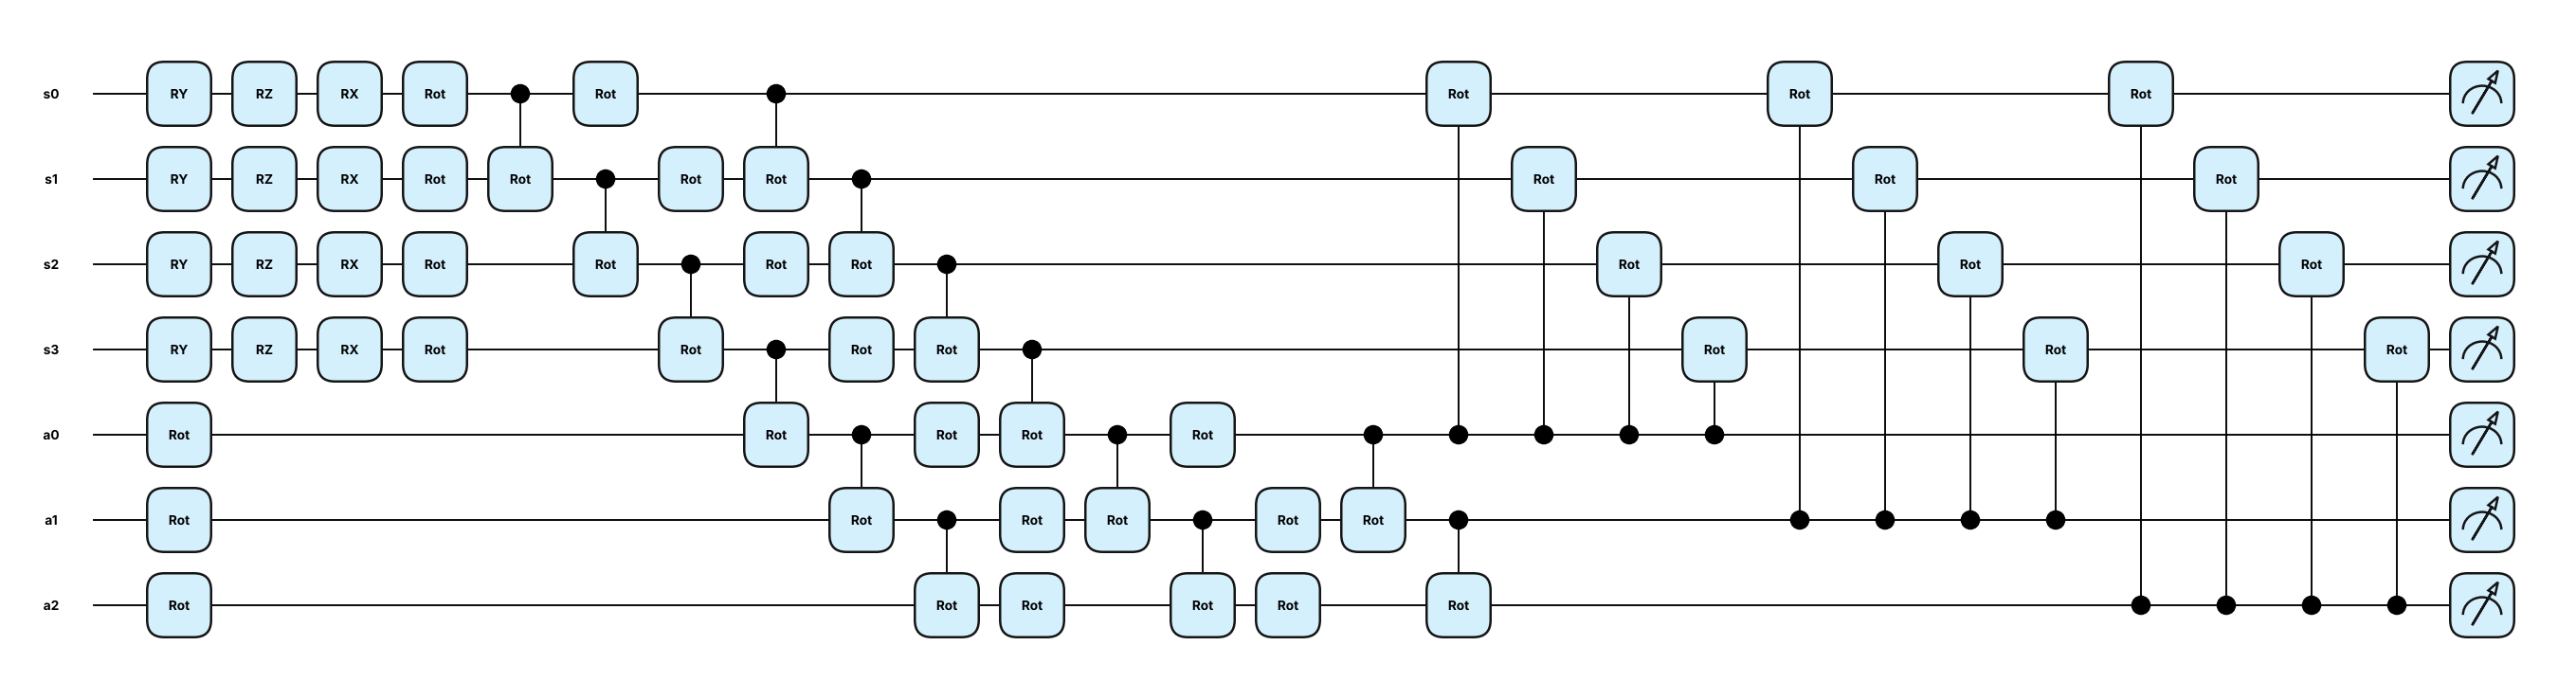
\includegraphics[width=\textwidth]{figures/circuit_one_patch.png}
  \caption{PennyLane drawing of the gates of one patch with $L=2$ repetitions of $W_i$ (the experiments use $L=2$ and $L=4$).}
  \label{fig:onepatch}
\end{figure}

\subsection{MNIST results}

Supplementary Tables~\ref{tab:mnist-results} and~\ref{tab:mnist-amp} give the test accuracies behind Figs.~\ref{fig:capacity} and~\ref{fig:classical}.

\begin{table}[htbp]
  \centering
  \caption{MNIST test accuracy (\%) at the last epoch, mean $\pm$ standard deviation over three seeds. Classical models are sized to the parameter count of the circuit with the given $L$; logistic regression does not depend on $L$. The best mean of each column within each block is in bold. $^\dagger$One of the three seeds stalled at about 47\% training accuracy and is included in the mean. Generated from the result files by \texttt{scripts/paper\_figures.py}.}
  \label{tab:mnist-results}
  \footnotesize
  \setlength{\tabcolsep}{3pt}
  \resizebox{\textwidth}{!}{\input{tables/mnist_results}}
\end{table}

\begin{table}[htbp]
  \centering
  \caption{MNIST test accuracy (\%) of the amplitude-encoding circuits: the whole image as a normalized amplitude vector of 4 qubits (shrunk to $4\times4$) or 7 qubits ($8\times8$ as it is, $14\times14$ shrunk to $11\times11$), followed by $L$ layers of the block of the serialized circuit and the same readout (60--462 parameters). Mean $\pm$ standard deviation over three seeds; the best mean of each column is in bold.}
  \label{tab:mnist-amp}
  \footnotesize
  \setlength{\tabcolsep}{3pt}
  \input{tables/mnist_amplitude}
\end{table}

\subsection{Twelve further datasets}

Supplementary Table~\ref{tab:datasets} describes the datasets and Supplementary Table~\ref{tab:bench} gives the test accuracies behind Fig.~\ref{fig:bench}.

\begin{table}[htbp]
  \centering
  \caption{The twelve further datasets. $d$: features, $N$: patches of four features, $k$: classes. Tabular sets keep their natural class frequencies (majority class in the last column); the image sets are class balanced except PneumoniaMNIST, which keeps its official splits.}
  \label{tab:datasets}
  \footnotesize
  \resizebox{\textwidth}{!}{%
  \begin{tabular}{@{}llrrrrr@{}}
    \toprule
    dataset & source & $d$ & $N$ & $k$ & train / val / test & majority \\
    \midrule
    Waveform & UCI 107~\cite{uci_waveform} (21 wave attributes) & 21 & 6 & 3 & 3\,601 / 400 / 999 & 33.9\% \\
    Wall-Following & UCI 194~\cite{freire2009wall}, 24 sensors & 24 & 6 & 4 & 3\,929 / 436 / 1\,091 & 40.4\% \\
    Covertype & UCI 31~\cite{uci_covertype,blackard1999covertype} & 54 & 14 & 7 & 10\,000 / 2\,000 / 9\,999 & 48.8\% \\
    Letter & UCI 59~\cite{frey1991letter} & 16 & 4 & 26 & 10\,000 / 1\,600 / 4\,000 & 4.1\% \\
    Spambase & UCI 94~\cite{uci_spambase} & 57 & 15 & 2 & 3\,313 / 368 / 920 & 60.5\% \\
    Credit Default & UCI 350~\cite{yeh2009credit} & 23 & 6 & 2 & 10\,000 / 2\,000 / 6\,000 & 77.9\% \\
    Landsat & UCI 146~\cite{uci_landsat,king1995statlog} (train and test joined) & 36 & 9 & 6 & 4\,634 / 514 / 1\,287 & 23.9\% \\
    Dry Bean & UCI 602~\cite{koklu2020drybean} & 16 & 4 & 7 & 9\,801 / 1\,089 / 2\,721 & 26.1\% \\
    \midrule
    Fashion-MNIST & \cite{xiao2017fashion}, $14\times14$ & 196 & 49 & 10 & 10\,000 / 2\,000 / 10\,000 & 10\% \\
    BloodMNIST & MedMNIST v2~\cite{yang2023medmnist,acevedo2020blood}, grayscale, $14\times14$ & 196 & 49 & 8 & 8\,779 / 1\,527 / 3\,421 & 19.5\% \\
    PneumoniaMNIST & MedMNIST v2~\cite{yang2023medmnist,kermany2018pneumonia}, $14\times14$ & 196 & 49 & 2 & 4\,708 / 524 / 624 & 62.5\% \\
    Kuzushiji-MNIST & \cite{clanuwat2018kmnist}, $14\times14$ & 196 & 49 & 10 & 10\,000 / 2\,000 / 10\,000 & 10\% \\
    \bottomrule
  \end{tabular}}
\end{table}

\begin{table}[htbp]
  \centering
  \caption{Test accuracy (\%) on twelve further datasets at the last epoch, mean $\pm$ standard deviation over three seeds; the best mean of each row is in bold. $k$: classes, $N$: patches of four features, params: parameters of the circuit with coherent memory and $L=4$, which is also the size of the MLP and the CNN. Amplitude: the whole input as the amplitude vector of the same seven qubits with $L=4$ or $8$ layers of the same block (200--550 parameters). Gradient boosting: scikit-learn histogram gradient boosting, an ensemble of 300 trees shown as a reference, not tuned. Measured memory was run on the tabular sets only (above the line).}
  \label{tab:bench}
  \footnotesize
  \setlength{\tabcolsep}{2.5pt}
  \resizebox{\textwidth}{!}{\input{tables/bench_results}}
\end{table}

\begin{table}[htbp]
  \centering
  \caption{As Supplementary Table~\ref{tab:bench}, but balanced accuracy (\%), the mean of the per-class recalls: last epoch, mean $\pm$ standard deviation over three seeds; the best mean of each row is in bold.}
  \label{tab:bench-bal}
  \footnotesize
  \setlength{\tabcolsep}{2.5pt}
  \resizebox{\textwidth}{!}{\input{tables/bench_balanced}}
\end{table}

\subsection{Classical models with the structure of the circuit}

\begin{table}[htbp]
  \centering
  \caption{The serialized circuit ($L=4$) against classical models that read the input patch by patch with position-specific parameters. Test accuracy (\%) at the last epoch, mean over three seeds; the best mean of each row is in bold. MLP: the one-hidden-layer MLP of Supplementary Table~\ref{tab:bench} (for MNIST, the parameter-matched MLP of Supplementary Table~\ref{tab:mnist-results}). Seq.\ RNN: recurrent network with its own weights at every patch; MPS: matrix-product-state classifier with one tensor per feature; both are sized to the parameter count of the circuit as closely as their hidden or bond dimension allows. 8-state HMM: input-driven hidden Markov model over eight states, with 1.5 to 2 times the parameters of the circuit. The learning rate of each classical model is chosen by mean validation accuracy. Measured memory was not run on the 49-patch image sets.}
  \label{tab:struct}
  \footnotesize
  \input{tables/struct_baselines}
\end{table}

\subsection{Readout and head variants on Letter}

Supplementary Table~\ref{tab:letter} collects the variants of the circuit run on Letter, each against a one-hidden-layer MLP with the same number of parameters.

\begin{table}[htbp]
  \centering
  \caption{Letter (26 classes): readout, head and depth variants of the circuit with coherent memory, against a one-hidden-layer MLP of the same size. Test accuracy (\%), mean $\pm$ standard deviation over three seeds; the better mean of each row is in bold. Gradient-boosted trees reach $95.3\pm0.1$.}
  \label{tab:letter}
  \footnotesize
  \input{tables/letter_variants}
\end{table}

\subsection{$28\times28$ images}
\label{sec:supp-28}

At $28\times28$ the serialized circuit has 196 patches and 74\% of them are empty (62\% at $14\times14$, 41\% at $8\times8$). With the settings of the MNIST experiments it stays at chance or only fits the training set, and the simulation takes about 47 minutes (3 vs.\ 5) to 2 hours (10 classes) per epoch, i.e.\ days per run, so it is not reported. The classical and amplitude-encoding baselines were run at $28\times28$ and are in the code repository.
 after \appendix.
\section{Supplementary Information}
\label{sec:supp}
\renewcommand{\thefigure}{S\arabic{figure}}
\renewcommand{\thetable}{S\arabic{table}}
\setcounter{figure}{0}
\setcounter{table}{0}

\subsection{Gates of one patch}

Supplementary Fig.~\ref{fig:onepatch} shows the gates acting on one patch, as drawn by PennyLane for $L=2$: the encoding rotations on the system qubits, the $\mathrm{Rot}$ layers and $\mathrm{CRot}$ chains of $W_i$, and $W_c$ with the controlled rotations from each ancilla to the system qubits.

\begin{figure}[h]
  \centering
  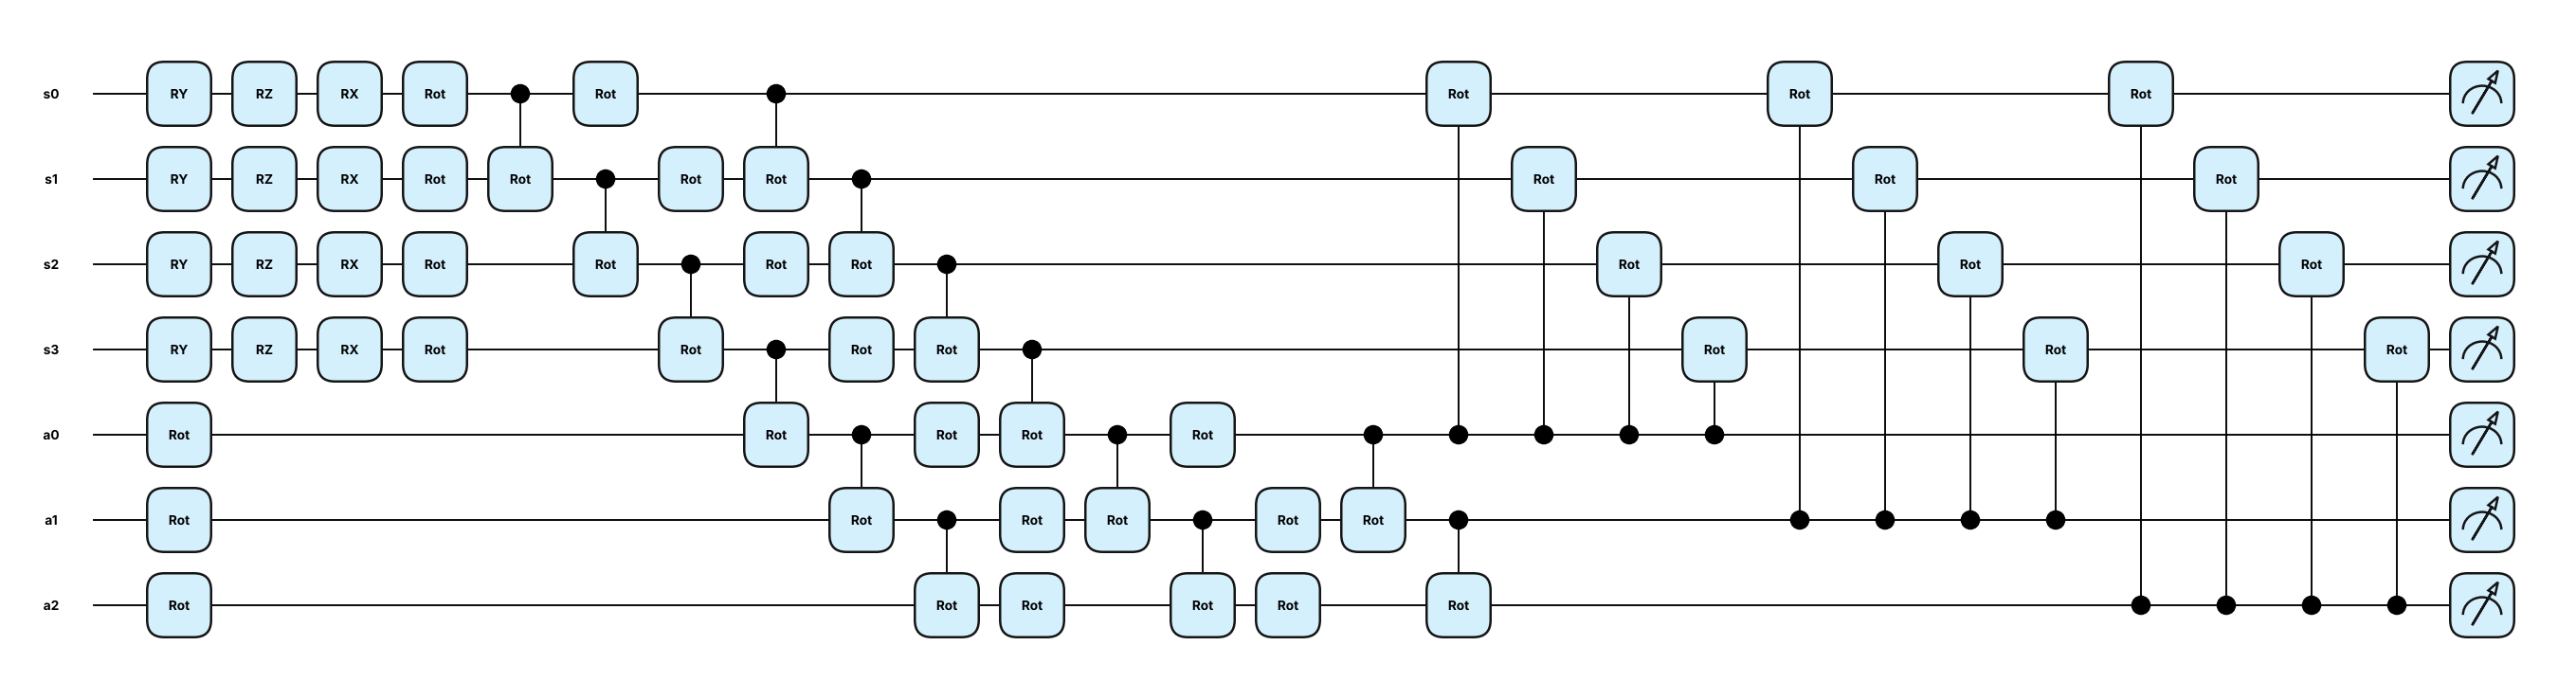
\includegraphics[width=\textwidth]{figures/circuit_one_patch.png}
  \caption{PennyLane drawing of the gates of one patch with $L=2$ repetitions of $W_i$ (the experiments use $L=2$ and $L=4$).}
  \label{fig:onepatch}
\end{figure}

\subsection{MNIST results}

Supplementary Tables~\ref{tab:mnist-results} and~\ref{tab:mnist-amp} give the test accuracies behind Figs.~\ref{fig:capacity} and~\ref{fig:classical}.

\begin{table}[htbp]
  \centering
  \caption{MNIST test accuracy (\%) at the last epoch, mean $\pm$ standard deviation over three seeds. Classical models are sized to the parameter count of the circuit with the given $L$; logistic regression does not depend on $L$. The best mean of each column within each block is in bold. $^\dagger$One of the three seeds stalled at about 47\% training accuracy and is included in the mean. Generated from the result files by \texttt{scripts/paper\_figures.py}.}
  \label{tab:mnist-results}
  \footnotesize
  \setlength{\tabcolsep}{3pt}
  \resizebox{\textwidth}{!}{% generated by scripts/paper_figures.py -- do not edit
\begin{tabular}{@{}lcccccccc@{}}
\toprule
 & \multicolumn{2}{c}{3 vs 5} & \multicolumn{2}{c}{4 vs 9} & \multicolumn{2}{c}{4 classes (0-3)} & \multicolumn{2}{c}{10 classes} \\
\cmidrule(lr){2-3}\cmidrule(lr){4-5}\cmidrule(lr){6-7}\cmidrule(lr){8-9}
 & $8{\times}8$ & $14{\times}14$ & $8{\times}8$ & $14{\times}14$ & $8{\times}8$ & $14{\times}14$ & $8{\times}8$ & $14{\times}14$ \\
\midrule
\multicolumn{9}{@{}l}{\emph{$L=2$ (classical models sized to the circuit with $L=2$)}} \\
serialized, coherent & $96.2\pm0.5$ & $96.9\pm0.2$ & $94.3\pm0.3$ & $96.3\pm0.5$ & $97.4\pm0.2$ & $97.7\pm0.2$ & $89.9\pm0.1$ & $91.8\pm0.2$ \\
serialized, measured & $95.7\pm0.5$ & $96.8\pm0.6$ & $92.6\pm0.4$ & $96.1\pm0.3$ & $90.7\pm4.8$ & $97.0\pm0.1$ & $64.0\pm14.1$$^\dagger$ & $79.9\pm2.8$ \\
MLP, same parameters & $95.6\pm0.1$ & $97.2\pm1.5$ & $95.8\pm0.1$ & $97.3\pm0.6$ & $97.7\pm0.3$ & $98.0\pm0.1$ & $92.0\pm0.2$ & $93.7\pm0.3$ \\
CNN, same parameters & $\mathbf{98.2}\pm0.2$ & $\mathbf{98.5}\pm0.3$ & $\mathbf{96.4}\pm0.2$ & $\mathbf{98.7}\pm0.2$ & $\mathbf{98.7}\pm0.1$ & $\mathbf{99.0}\pm0.1$ & $\mathbf{93.6}\pm0.5$ & $\mathbf{96.3}\pm0.1$ \\
logistic regression & $95.1\pm0.2$ & $95.7\pm0.5$ & $94.8\pm0.2$ & $97.0\pm0.3$ & $97.1\pm0.1$ & $97.5\pm0.1$ & $89.9\pm0.1$ & $91.7\pm0.1$ \\
\midrule
\multicolumn{9}{@{}l}{\emph{$L=4$ (classical models sized to the circuit with $L=4$)}} \\
serialized, coherent & $97.2\pm0.3$ & $97.5\pm0.2$ & $94.9\pm0.3$ & $97.0\pm0.6$ & $97.0\pm0.1$ & $97.8\pm0.3$ & $91.1\pm0.3$ & $92.8\pm0.4$ \\
serialized, measured & $96.9\pm0.2$ & $97.0\pm0.6$ & $94.8\pm0.4$ & $96.8\pm0.3$ & $96.3\pm0.6$ & $97.5\pm0.2$ & $81.2\pm4.1$ & $86.2\pm3.3$ \\
MLP, same parameters & $97.7\pm0.7$ & $98.0\pm0.6$ & $96.8\pm0.3$ & $97.7\pm0.4$ & $98.3\pm0.2$ & $98.3\pm0.0$ & $94.7\pm0.3$ & $95.1\pm0.1$ \\
CNN, same parameters & $\mathbf{98.4}\pm0.4$ & $\mathbf{98.7}\pm0.1$ & $\mathbf{97.0}\pm0.4$ & $\mathbf{98.9}\pm0.2$ & $\mathbf{98.8}\pm0.0$ & $\mathbf{99.1}\pm0.1$ & $\mathbf{95.3}\pm0.2$ & $\mathbf{97.2}\pm0.2$ \\
\bottomrule
\end{tabular}
}
\end{table}

\begin{table}[htbp]
  \centering
  \caption{MNIST test accuracy (\%) of the amplitude-encoding circuits: the whole image as a normalized amplitude vector of 4 qubits (shrunk to $4\times4$) or 7 qubits ($8\times8$ as it is, $14\times14$ shrunk to $11\times11$), followed by $L$ layers of the block of the serialized circuit and the same readout (60--462 parameters). Mean $\pm$ standard deviation over three seeds; the best mean of each column is in bold.}
  \label{tab:mnist-amp}
  \footnotesize
  \setlength{\tabcolsep}{3pt}
  % generated by scripts/paper_figures.py -- do not edit
\begin{tabular}{@{}llcccccccc@{}}
\toprule
 & & \multicolumn{2}{c}{3 vs 5} & \multicolumn{2}{c}{4 vs 9} & \multicolumn{2}{c}{4 classes (0-3)} & \multicolumn{2}{c}{10 classes} \\
\cmidrule(lr){3-4}\cmidrule(lr){5-6}\cmidrule(lr){7-8}\cmidrule(lr){9-10}
qubits & $L$ & $8{\times}8$ & $14{\times}14$ & $8{\times}8$ & $14{\times}14$ & $8{\times}8$ & $14{\times}14$ & $8{\times}8$ & $14{\times}14$ \\
\midrule
4 & 2 & $93.6\pm0.7$ & $93.8\pm0.4$ & $78.0\pm0.6$ & $83.5\pm0.3$ & $88.7\pm0.1$ & $89.2\pm1.1$ & $68.8\pm0.1$ & $72.1\pm1.4$ \\
4 & 4 & $93.9\pm0.2$ & $94.6\pm0.2$ & $79.0\pm1.8$ & $85.0\pm0.4$ & $89.1\pm0.3$ & $90.6\pm0.1$ & $70.5\pm0.7$ & $75.6\pm0.6$ \\
4 & 8 & $94.4\pm0.4$ & $94.6\pm0.2$ & $79.7\pm0.5$ & $85.3\pm1.0$ & $90.0\pm0.4$ & $90.9\pm0.4$ & $72.4\pm0.3$ & $76.4\pm0.9$ \\
\midrule
7 & 2 & $93.5\pm1.4$ & $92.3\pm0.2$ & $88.4\pm0.4$ & $94.9\pm0.4$ & $96.0\pm0.2$ & $96.0\pm0.1$ & $82.4\pm1.2$ & $82.9\pm1.5$ \\
7 & 4 & $94.9\pm1.0$ & $94.6\pm0.8$ & $90.2\pm0.1$ & $\mathbf{95.2}\pm0.1$ & $96.6\pm0.4$ & $96.8\pm0.4$ & $86.3\pm0.2$ & $86.4\pm1.0$ \\
7 & 8 & $\mathbf{96.0}\pm0.5$ & $\mathbf{95.7}\pm0.5$ & $\mathbf{93.5}\pm0.6$ & $\mathbf{95.2}\pm0.5$ & $\mathbf{97.5}\pm0.2$ & $\mathbf{97.1}\pm0.2$ & $\mathbf{87.9}\pm0.4$ & $\mathbf{89.2}\pm0.5$ \\
\bottomrule
\end{tabular}

\end{table}

\subsection{Twelve further datasets}

Supplementary Table~\ref{tab:datasets} describes the datasets and Supplementary Table~\ref{tab:bench} gives the test accuracies behind Fig.~\ref{fig:bench}.

\begin{table}[htbp]
  \centering
  \caption{The twelve further datasets. $d$: features, $N$: patches of four features, $k$: classes. Tabular sets keep their natural class frequencies (majority class in the last column); the image sets are class balanced except PneumoniaMNIST, which keeps its official splits.}
  \label{tab:datasets}
  \footnotesize
  \resizebox{\textwidth}{!}{%
  \begin{tabular}{@{}llrrrrr@{}}
    \toprule
    dataset & source & $d$ & $N$ & $k$ & train / val / test & majority \\
    \midrule
    Waveform & UCI 107~\cite{uci_waveform} (21 wave attributes) & 21 & 6 & 3 & 3\,601 / 400 / 999 & 33.9\% \\
    Wall-Following & UCI 194~\cite{freire2009wall}, 24 sensors & 24 & 6 & 4 & 3\,929 / 436 / 1\,091 & 40.4\% \\
    Covertype & UCI 31~\cite{uci_covertype,blackard1999covertype} & 54 & 14 & 7 & 10\,000 / 2\,000 / 9\,999 & 48.8\% \\
    Letter & UCI 59~\cite{frey1991letter} & 16 & 4 & 26 & 10\,000 / 1\,600 / 4\,000 & 4.1\% \\
    Spambase & UCI 94~\cite{uci_spambase} & 57 & 15 & 2 & 3\,313 / 368 / 920 & 60.5\% \\
    Credit Default & UCI 350~\cite{yeh2009credit} & 23 & 6 & 2 & 10\,000 / 2\,000 / 6\,000 & 77.9\% \\
    Landsat & UCI 146~\cite{uci_landsat,king1995statlog} (train and test joined) & 36 & 9 & 6 & 4\,634 / 514 / 1\,287 & 23.9\% \\
    Dry Bean & UCI 602~\cite{koklu2020drybean} & 16 & 4 & 7 & 9\,801 / 1\,089 / 2\,721 & 26.1\% \\
    \midrule
    Fashion-MNIST & \cite{xiao2017fashion}, $14\times14$ & 196 & 49 & 10 & 10\,000 / 2\,000 / 10\,000 & 10\% \\
    BloodMNIST & MedMNIST v2~\cite{yang2023medmnist,acevedo2020blood}, grayscale, $14\times14$ & 196 & 49 & 8 & 8\,779 / 1\,527 / 3\,421 & 19.5\% \\
    PneumoniaMNIST & MedMNIST v2~\cite{yang2023medmnist,kermany2018pneumonia}, $14\times14$ & 196 & 49 & 2 & 4\,708 / 524 / 624 & 62.5\% \\
    Kuzushiji-MNIST & \cite{clanuwat2018kmnist}, $14\times14$ & 196 & 49 & 10 & 10\,000 / 2\,000 / 10\,000 & 10\% \\
    \bottomrule
  \end{tabular}}
\end{table}

\begin{table}[htbp]
  \centering
  \caption{Test accuracy (\%) on twelve further datasets at the last epoch, mean $\pm$ standard deviation over three seeds; the best mean of each row is in bold. $k$: classes, $N$: patches of four features, params: parameters of the circuit with coherent memory and $L=4$, which is also the size of the MLP and the CNN. Amplitude: the whole input as the amplitude vector of the same seven qubits with $L=4$ or $8$ layers of the same block (200--550 parameters). Gradient boosting: scikit-learn histogram gradient boosting, an ensemble of 300 trees shown as a reference, not tuned. Measured memory was run on the tabular sets only (above the line).}
  \label{tab:bench}
  \footnotesize
  \setlength{\tabcolsep}{2.5pt}
  \resizebox{\textwidth}{!}{% generated by scripts/paper_figures.py -- do not edit
\begin{tabular}{@{}lrrrrrrrrrrr@{}}
\toprule
 & & & & \multicolumn{4}{c}{classical} & \multicolumn{2}{c}{amplitude, 7 qubits} & \multicolumn{2}{c@{}}{serialized, 7 qubits} \\
\cmidrule(lr){5-8}\cmidrule(lr){9-10}\cmidrule(l){11-12}
dataset & $k$ & $N$ & params & logistic & MLP & CNN & grad.\ boost. & $L{=}4$ & $L{=}8$ & \multicolumn{1}{c}{coherent} & \multicolumn{1}{c@{}}{measured} \\
\midrule
Waveform & 3 & 6 & 1056 & $\mathbf{87.2}${\scriptsize$\pm0.1$} & $87.1${\scriptsize$\pm0.8$} & -- & $85.5${\scriptsize$\pm0.5$} & $86.2${\scriptsize$\pm0.2$} & $86.8${\scriptsize$\pm0.6$} & $85.0${\scriptsize$\pm0.2$} & $82.7${\scriptsize$\pm3.1$} \\
Wall-Following & 4 & 6 & 1071 & $68.3${\scriptsize$\pm0.3$} & $91.9${\scriptsize$\pm0.4$} & -- & $\mathbf{99.9}${\scriptsize$\pm0.0$} & $73.0${\scriptsize$\pm1.4$} & $77.1${\scriptsize$\pm1.5$} & $90.1${\scriptsize$\pm0.7$} & $87.0${\scriptsize$\pm2.0$} \\
Covertype & 7 & 14 & 2364 & $71.6${\scriptsize$\pm0.1$} & $75.8${\scriptsize$\pm0.2$} & -- & $\mathbf{82.2}${\scriptsize$\pm0.2$} & $71.7${\scriptsize$\pm0.5$} & $72.0${\scriptsize$\pm0.3$} & $73.8${\scriptsize$\pm0.2$} & $71.7${\scriptsize$\pm0.5$} \\
Letter & 26 & 4 & 1089 & $72.6${\scriptsize$\pm0.2$} & $80.4${\scriptsize$\pm0.8$} & -- & $\mathbf{95.3}${\scriptsize$\pm0.1$} & $59.7${\scriptsize$\pm2.5$} & $63.6${\scriptsize$\pm0.8$} & $71.0${\scriptsize$\pm1.6$} & $63.5${\scriptsize$\pm3.1$} \\
Spambase & 2 & 15 & 2445 & $92.0${\scriptsize$\pm0.1$} & $93.4${\scriptsize$\pm0.5$} & -- & $\mathbf{96.1}${\scriptsize$\pm0.3$} & $90.0${\scriptsize$\pm0.4$} & $90.7${\scriptsize$\pm0.8$} & $91.7${\scriptsize$\pm0.4$} & $93.5${\scriptsize$\pm0.6$} \\
Credit Default & 2 & 6 & 1041 & $81.1${\scriptsize$\pm0.1$} & $81.7${\scriptsize$\pm0.1$} & -- & $81.4${\scriptsize$\pm0.3$} & $79.6${\scriptsize$\pm0.2$} & $79.7${\scriptsize$\pm0.1$} & $81.9${\scriptsize$\pm0.3$} & $\mathbf{82.4}${\scriptsize$\pm0.1$} \\
Landsat & 6 & 9 & 1569 & $82.3${\scriptsize$\pm0.2$} & $89.2${\scriptsize$\pm0.1$} & -- & $\mathbf{92.3}${\scriptsize$\pm0.5$} & $78.7${\scriptsize$\pm0.2$} & $78.9${\scriptsize$\pm0.2$} & $89.3${\scriptsize$\pm1.2$} & $86.8${\scriptsize$\pm1.0$} \\
Dry Bean & 7 & 4 & 804 & $92.1${\scriptsize$\pm0.0$} & $92.3${\scriptsize$\pm0.1$} & -- & $92.8${\scriptsize$\pm0.2$} & $91.8${\scriptsize$\pm0.1$} & $91.8${\scriptsize$\pm0.2$} & $\mathbf{92.9}${\scriptsize$\pm0.2$} & $92.8${\scriptsize$\pm0.0$} \\
\midrule
Fashion-MNIST & 10 & 49 & 7869 & $82.6${\scriptsize$\pm0.2$} & $85.2${\scriptsize$\pm0.1$} & $85.7${\scriptsize$\pm0.6$} & $\mathbf{86.5}${\scriptsize$\pm0.4$} & $73.7${\scriptsize$\pm0.4$} & $74.4${\scriptsize$\pm0.8$} & $82.7${\scriptsize$\pm0.2$} & -- \\
BloodMNIST & 8 & 49 & 7839 & $67.2${\scriptsize$\pm0.4$} & $70.3${\scriptsize$\pm1.2$} & $81.2${\scriptsize$\pm0.4$} & $\mathbf{86.0}${\scriptsize$\pm0.2$} & $58.0${\scriptsize$\pm0.6$} & $60.2${\scriptsize$\pm0.2$} & $73.8${\scriptsize$\pm1.3$} & -- \\
PneumoniaMNIST & 2 & 49 & 7749 & $83.5${\scriptsize$\pm0.1$} & $84.1${\scriptsize$\pm0.9$} & $85.6${\scriptsize$\pm0.8$} & $84.9${\scriptsize$\pm0.0$} & $81.2${\scriptsize$\pm1.5$} & $81.9${\scriptsize$\pm1.2$} & $\mathbf{87.7}${\scriptsize$\pm0.7$} & -- \\
Kuzushiji-MNIST & 10 & 49 & 7869 & $68.2${\scriptsize$\pm0.3$} & $78.7${\scriptsize$\pm0.2$} & $80.3${\scriptsize$\pm1.5$} & $\mathbf{83.4}${\scriptsize$\pm0.3$} & $58.3${\scriptsize$\pm0.8$} & $62.6${\scriptsize$\pm0.8$} & $70.4${\scriptsize$\pm0.7$} & -- \\
\bottomrule
\end{tabular}
}
\end{table}

\begin{table}[htbp]
  \centering
  \caption{As Supplementary Table~\ref{tab:bench}, but balanced accuracy (\%), the mean of the per-class recalls: last epoch, mean $\pm$ standard deviation over three seeds; the best mean of each row is in bold.}
  \label{tab:bench-bal}
  \footnotesize
  \setlength{\tabcolsep}{2.5pt}
  \resizebox{\textwidth}{!}{% generated by scripts/paper_figures.py -- do not edit
\begin{tabular}{@{}lrrrrrrrrrrr@{}}
\toprule
 & & & & \multicolumn{4}{c}{classical} & \multicolumn{2}{c}{amplitude, 7 qubits} & \multicolumn{2}{c@{}}{serialized, 7 qubits} \\
\cmidrule(lr){5-8}\cmidrule(lr){9-10}\cmidrule(l){11-12}
dataset & $k$ & $N$ & params & logistic & MLP & CNN & grad.\ boost. & $L{=}4$ & $L{=}8$ & \multicolumn{1}{c}{coherent} & \multicolumn{1}{c@{}}{measured} \\
\midrule
Waveform & 3 & 6 & 1056 & $\mathbf{87.2}${\scriptsize$\pm0.1$} & $87.1${\scriptsize$\pm0.8$} & -- & $85.5${\scriptsize$\pm0.5$} & $86.2${\scriptsize$\pm0.2$} & $86.8${\scriptsize$\pm0.6$} & $85.0${\scriptsize$\pm0.2$} & $82.7${\scriptsize$\pm3.1$} \\
Wall-Following & 4 & 6 & 1071 & $59.7${\scriptsize$\pm1.0$} & $90.8${\scriptsize$\pm0.9$} & -- & $\mathbf{99.9}${\scriptsize$\pm0.0$} & $66.2${\scriptsize$\pm1.8$} & $69.9${\scriptsize$\pm0.9$} & $88.8${\scriptsize$\pm0.8$} & $84.6${\scriptsize$\pm2.7$} \\
Covertype & 7 & 14 & 2364 & $46.0${\scriptsize$\pm1.2$} & $56.2${\scriptsize$\pm2.4$} & -- & $\mathbf{67.8}${\scriptsize$\pm0.2$} & $42.3${\scriptsize$\pm0.1$} & $42.1${\scriptsize$\pm1.7$} & $45.3${\scriptsize$\pm1.2$} & $38.1${\scriptsize$\pm2.6$} \\
Letter & 26 & 4 & 1089 & $72.5${\scriptsize$\pm0.2$} & $80.4${\scriptsize$\pm0.8$} & -- & $\mathbf{95.3}${\scriptsize$\pm0.1$} & $59.6${\scriptsize$\pm2.4$} & $63.5${\scriptsize$\pm0.7$} & $70.8${\scriptsize$\pm1.6$} & $63.5${\scriptsize$\pm3.1$} \\
Spambase & 2 & 15 & 2445 & $91.2${\scriptsize$\pm0.1$} & $92.9${\scriptsize$\pm0.4$} & -- & $\mathbf{96.1}${\scriptsize$\pm0.3$} & $89.2${\scriptsize$\pm0.5$} & $90.0${\scriptsize$\pm0.8$} & $91.4${\scriptsize$\pm0.8$} & $93.1${\scriptsize$\pm0.7$} \\
Credit Default & 2 & 6 & 1041 & $61.2${\scriptsize$\pm0.2$} & $65.4${\scriptsize$\pm0.3$} & -- & $65.0${\scriptsize$\pm0.2$} & $58.5${\scriptsize$\pm0.4$} & $59.1${\scriptsize$\pm0.3$} & $65.3${\scriptsize$\pm0.7$} & $\mathbf{66.3}${\scriptsize$\pm0.4$} \\
Landsat & 6 & 9 & 1569 & $74.7${\scriptsize$\pm0.4$} & $86.5${\scriptsize$\pm0.1$} & -- & $\mathbf{90.1}${\scriptsize$\pm0.6$} & $69.3${\scriptsize$\pm0.2$} & $69.4${\scriptsize$\pm0.2$} & $86.8${\scriptsize$\pm1.4$} & $83.6${\scriptsize$\pm1.3$} \\
Dry Bean & 7 & 4 & 804 & $93.4${\scriptsize$\pm0.0$} & $93.5${\scriptsize$\pm0.0$} & -- & $93.8${\scriptsize$\pm0.2$} & $92.9${\scriptsize$\pm0.2$} & $93.0${\scriptsize$\pm0.1$} & $\mathbf{93.9}${\scriptsize$\pm0.2$} & $93.8${\scriptsize$\pm0.1$} \\
\midrule
Fashion-MNIST & 10 & 49 & 7869 & $82.6${\scriptsize$\pm0.2$} & $85.2${\scriptsize$\pm0.1$} & $85.7${\scriptsize$\pm0.6$} & $\mathbf{86.5}${\scriptsize$\pm0.4$} & $73.7${\scriptsize$\pm0.4$} & $74.4${\scriptsize$\pm0.8$} & $82.7${\scriptsize$\pm0.2$} & -- \\
BloodMNIST & 8 & 49 & 7839 & $67.2${\scriptsize$\pm0.4$} & $69.8${\scriptsize$\pm1.1$} & $79.5${\scriptsize$\pm0.4$} & $\mathbf{84.8}${\scriptsize$\pm0.3$} & $55.5${\scriptsize$\pm0.5$} & $57.4${\scriptsize$\pm1.1$} & $73.0${\scriptsize$\pm1.1$} & -- \\
PneumoniaMNIST & 2 & 49 & 7749 & $78.9${\scriptsize$\pm0.2$} & $79.3${\scriptsize$\pm1.4$} & $81.2${\scriptsize$\pm1.2$} & $80.8${\scriptsize$\pm0.0$} & $76.1${\scriptsize$\pm2.1$} & $77.0${\scriptsize$\pm1.8$} & $\mathbf{84.0}${\scriptsize$\pm1.0$} & -- \\
Kuzushiji-MNIST & 10 & 49 & 7869 & $68.2${\scriptsize$\pm0.3$} & $78.7${\scriptsize$\pm0.2$} & $80.3${\scriptsize$\pm1.5$} & $\mathbf{83.4}${\scriptsize$\pm0.3$} & $58.3${\scriptsize$\pm0.8$} & $62.6${\scriptsize$\pm0.8$} & $70.4${\scriptsize$\pm0.7$} & -- \\
\bottomrule
\end{tabular}
}
\end{table}

\subsection{Classical models with the structure of the circuit}

\begin{table}[htbp]
  \centering
  \caption{The serialized circuit ($L=4$) against classical models that read the input patch by patch with position-specific parameters. Test accuracy (\%) at the last epoch, mean over three seeds; the best mean of each row is in bold. MLP: the one-hidden-layer MLP of Supplementary Table~\ref{tab:bench} (for MNIST, the parameter-matched MLP of Supplementary Table~\ref{tab:mnist-results}). Seq.\ RNN: recurrent network with its own weights at every patch; MPS: matrix-product-state classifier with one tensor per feature; both are sized to the parameter count of the circuit as closely as their hidden or bond dimension allows. 8-state HMM: input-driven hidden Markov model over eight states, with 1.5 to 2 times the parameters of the circuit. The learning rate of each classical model is chosen by mean validation accuracy. Measured memory was not run on the 49-patch image sets.}
  \label{tab:struct}
  \footnotesize
  % generated by scripts/paper_figures.py -- do not edit
\begin{tabular}{@{}lrrrrrr@{}}
\toprule
 & \multicolumn{2}{c}{serialized circuit} & \multicolumn{4}{c@{}}{classical} \\
\cmidrule(lr){2-3}\cmidrule(l){4-7}
dataset & coherent & measured & MLP & seq.\ RNN & MPS & 8-state HMM \\
\midrule
Waveform & $85.0$ & $82.7$ & $87.1$ & $87.4$ & $\mathbf{87.5}$ & $84.9$ \\
Wall-Following & $90.1$ & $87.0$ & $91.9$ & $93.1$ & $\mathbf{95.2}$ & $85.7$ \\
Covertype & $73.8$ & $71.7$ & $\mathbf{75.8}$ & $75.3$ & $75.2$ & $71.3$ \\
Letter & $71.0$ & $63.5$ & $80.4$ & $\mathbf{80.7}$ & $71.4$ & $53.8$ \\
Spambase & $91.7$ & $93.5$ & $93.4$ & $93.2$ & $\mathbf{93.8}$ & $92.5$ \\
Credit Default & $81.9$ & $\mathbf{82.4}$ & $81.7$ & $82.2$ & $82.0$ & $81.9$ \\
Landsat & $89.3$ & $86.8$ & $89.2$ & $\mathbf{89.7}$ & $89.6$ & $83.7$ \\
Dry Bean & $\mathbf{92.9}$ & $92.8$ & $92.3$ & $92.8$ & $\mathbf{92.9}$ & $91.9$ \\
Fashion-MNIST & $82.7$ & -- & $\mathbf{85.2}$ & $77.1$ & $82.2$ & $53.0$ \\
BloodMNIST & $\mathbf{73.8}$ & -- & $70.3$ & $64.7$ & $71.9$ & $44.9$ \\
PneumoniaMNIST & $\mathbf{87.7}$ & -- & $84.1$ & $87.6$ & $87.5$ & $82.9$ \\
Kuzushiji-MNIST & $70.4$ & -- & $\mathbf{78.7}$ & $61.8$ & $62.1$ & $31.0$ \\
MNIST $8\times8$, 3 vs.\ 5 & $97.2$ & $96.9$ & $97.7$ & $\mathbf{98.1}$ & $97.4$ & $65.0$ \\
MNIST $8\times8$, 10 classes & $91.1$ & $81.2$ & $\mathbf{94.7}$ & $92.7$ & $92.1$ & $68.2$ \\
\bottomrule
\end{tabular}

\end{table}

\subsection{Readout and head variants on Letter}

Supplementary Table~\ref{tab:letter} collects the variants of the circuit run on Letter, each against a one-hidden-layer MLP with the same number of parameters.

\begin{table}[htbp]
  \centering
  \caption{Letter (26 classes): readout, head and depth variants of the circuit with coherent memory, against a one-hidden-layer MLP of the same size. Test accuracy (\%), mean $\pm$ standard deviation over three seeds; the better mean of each row is in bold. Gradient-boosted trees reach $95.3\pm0.1$.}
  \label{tab:letter}
  \footnotesize
  % generated by scripts/paper_figures.py -- do not edit
\begin{tabular}{@{}lrlrl@{}}
\toprule
 & \multicolumn{2}{c}{circuit} & \multicolumn{2}{c@{}}{MLP, same size} \\
\cmidrule(lr){2-3}\cmidrule(l){4-5}
readout and head & params & accuracy & params & accuracy \\
\midrule
$Z$, $ZZ$ (14 features), linear head, $L=4$ & 1\,089 & $71.0\pm1.6$ & 1\,101 & $\mathbf{80.4}\pm0.8$ \\
$Z$, $ZZ$ (14 features), linear head, $L=9$ & 1\,869 & $71.8\pm2.1$ & -- & -- \\
$+X$, $XX$, $Y$, $YY$ (42 features), linear head, $L=4$ & 1\,817 & $79.9\pm0.2$ & 1\,832 & $\mathbf{84.7}\pm1.2$ \\
$Z$, $ZZ$ (14 features), MLP head (64 units), $L=4$ & 3\,349 & $85.6\pm0.6$ & 3\,337 & $\mathbf{87.8}\pm0.2$ \\
\bottomrule
\end{tabular}

\end{table}

\subsection{$28\times28$ images}
\label{sec:supp-28}

At $28\times28$ the serialized circuit has 196 patches and 74\% of them are empty (62\% at $14\times14$, 41\% at $8\times8$). With the settings of the MNIST experiments it stays at chance or only fits the training set, and the simulation takes about 47 minutes (3 vs.\ 5) to 2 hours (10 classes) per epoch, i.e.\ days per run, so it is not reported. The classical and amplitude-encoding baselines were run at $28\times28$ and are in the code repository.
 after \appendix.
\section{Supplementary Information}
\label{sec:supp}
\renewcommand{\thefigure}{S\arabic{figure}}
\renewcommand{\thetable}{S\arabic{table}}
\setcounter{figure}{0}
\setcounter{table}{0}

\subsection{Gates of one patch}

Supplementary Fig.~\ref{fig:onepatch} shows the gates acting on one patch, as drawn by PennyLane for $L=2$: the encoding rotations on the system qubits, the $\mathrm{Rot}$ layers and $\mathrm{CRot}$ chains of $W_i$, and $W_c$ with the controlled rotations from each ancilla to the system qubits.

\begin{figure}[h]
  \centering
  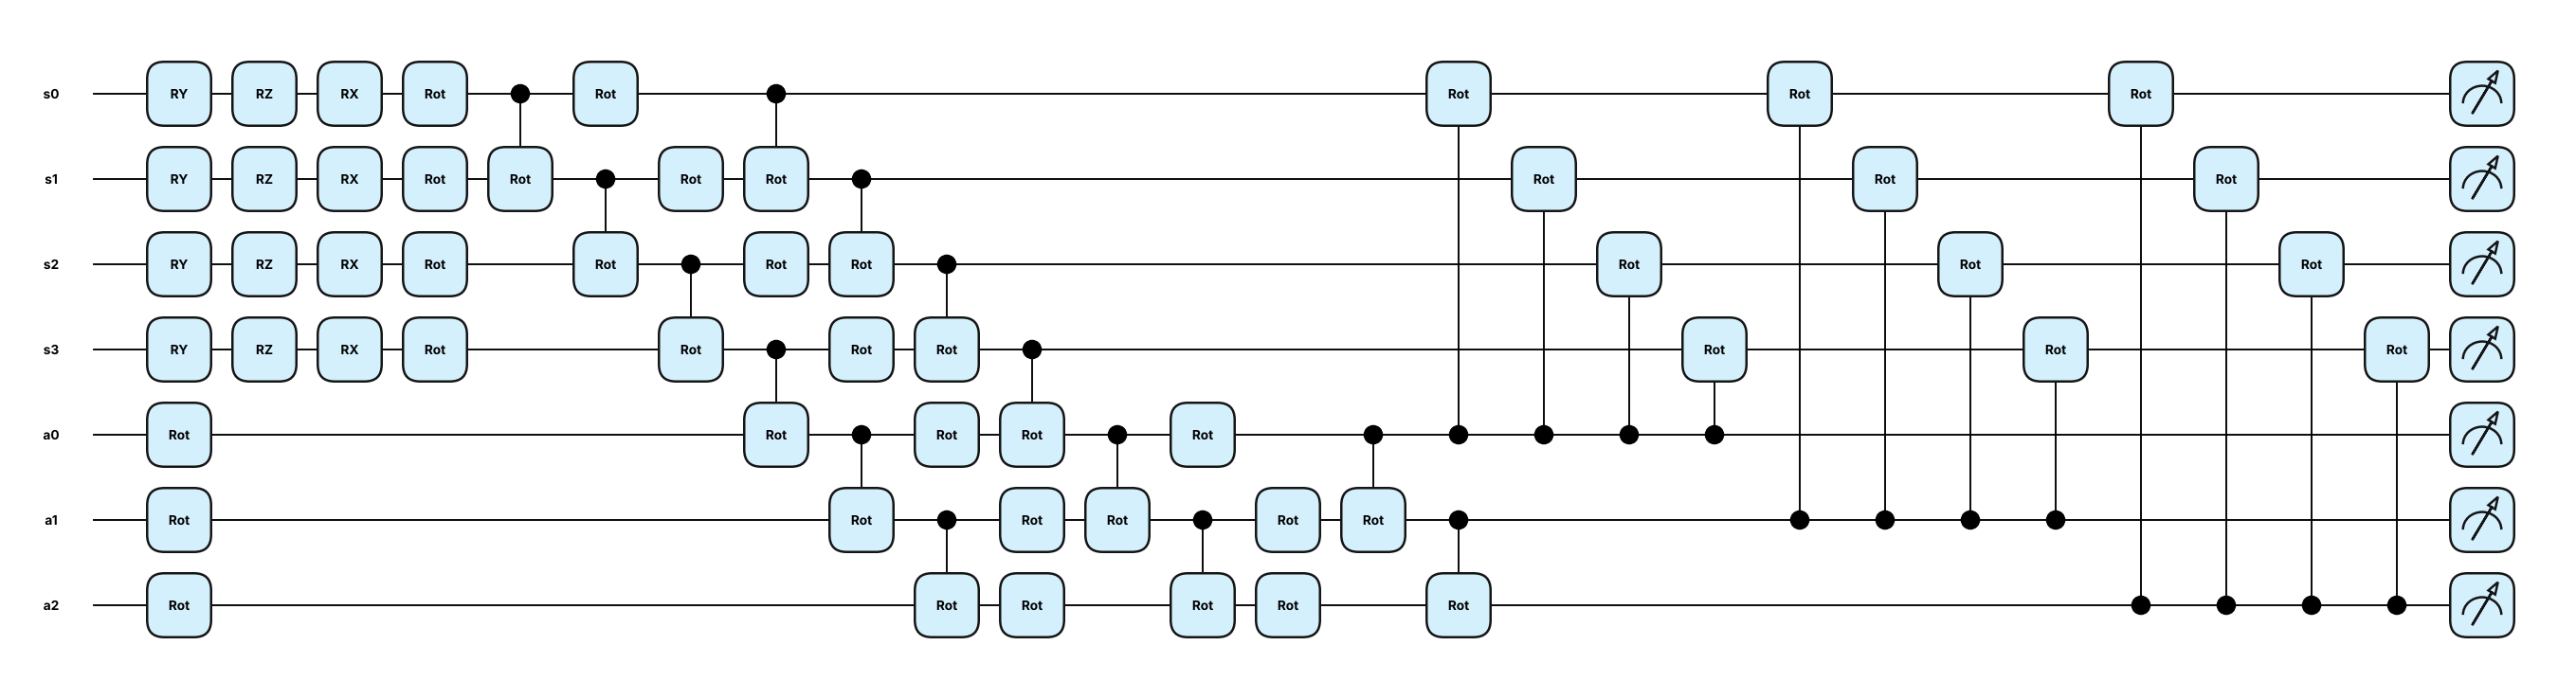
\includegraphics[width=\textwidth]{figures/circuit_one_patch.png}
  \caption{PennyLane drawing of the gates of one patch with $L=2$ repetitions of $W_i$ (the experiments use $L=2$ and $L=4$).}
  \label{fig:onepatch}
\end{figure}

\subsection{MNIST results}

Supplementary Tables~\ref{tab:mnist-results} and~\ref{tab:mnist-amp} give the test accuracies behind Figs.~\ref{fig:capacity} and~\ref{fig:classical}.

\begin{table}[htbp]
  \centering
  \caption{MNIST test accuracy (\%) at the last epoch, mean $\pm$ standard deviation over three seeds. Classical models are sized to the parameter count of the circuit with the given $L$; logistic regression does not depend on $L$. The best mean of each column within each block is in bold. $^\dagger$One of the three seeds stalled at about 47\% training accuracy and is included in the mean. Generated from the result files by \texttt{scripts/paper\_figures.py}.}
  \label{tab:mnist-results}
  \footnotesize
  \setlength{\tabcolsep}{3pt}
  \resizebox{\textwidth}{!}{% generated by scripts/paper_figures.py -- do not edit
\begin{tabular}{@{}lcccccccc@{}}
\toprule
 & \multicolumn{2}{c}{3 vs 5} & \multicolumn{2}{c}{4 vs 9} & \multicolumn{2}{c}{4 classes (0-3)} & \multicolumn{2}{c}{10 classes} \\
\cmidrule(lr){2-3}\cmidrule(lr){4-5}\cmidrule(lr){6-7}\cmidrule(lr){8-9}
 & $8{\times}8$ & $14{\times}14$ & $8{\times}8$ & $14{\times}14$ & $8{\times}8$ & $14{\times}14$ & $8{\times}8$ & $14{\times}14$ \\
\midrule
\multicolumn{9}{@{}l}{\emph{$L=2$ (classical models sized to the circuit with $L=2$)}} \\
serialized, coherent & $96.2\pm0.5$ & $96.9\pm0.2$ & $94.3\pm0.3$ & $96.3\pm0.5$ & $97.4\pm0.2$ & $97.7\pm0.2$ & $89.9\pm0.1$ & $91.8\pm0.2$ \\
serialized, measured & $95.7\pm0.5$ & $96.8\pm0.6$ & $92.6\pm0.4$ & $96.1\pm0.3$ & $90.7\pm4.8$ & $97.0\pm0.1$ & $64.0\pm14.1$$^\dagger$ & $79.9\pm2.8$ \\
MLP, same parameters & $95.6\pm0.1$ & $97.2\pm1.5$ & $95.8\pm0.1$ & $97.3\pm0.6$ & $97.7\pm0.3$ & $98.0\pm0.1$ & $92.0\pm0.2$ & $93.7\pm0.3$ \\
CNN, same parameters & $\mathbf{98.2}\pm0.2$ & $\mathbf{98.5}\pm0.3$ & $\mathbf{96.4}\pm0.2$ & $\mathbf{98.7}\pm0.2$ & $\mathbf{98.7}\pm0.1$ & $\mathbf{99.0}\pm0.1$ & $\mathbf{93.6}\pm0.5$ & $\mathbf{96.3}\pm0.1$ \\
logistic regression & $95.1\pm0.2$ & $95.7\pm0.5$ & $94.8\pm0.2$ & $97.0\pm0.3$ & $97.1\pm0.1$ & $97.5\pm0.1$ & $89.9\pm0.1$ & $91.7\pm0.1$ \\
\midrule
\multicolumn{9}{@{}l}{\emph{$L=4$ (classical models sized to the circuit with $L=4$)}} \\
serialized, coherent & $97.2\pm0.3$ & $97.5\pm0.2$ & $94.9\pm0.3$ & $97.0\pm0.6$ & $97.0\pm0.1$ & $97.8\pm0.3$ & $91.1\pm0.3$ & $92.8\pm0.4$ \\
serialized, measured & $96.9\pm0.2$ & $97.0\pm0.6$ & $94.8\pm0.4$ & $96.8\pm0.3$ & $96.3\pm0.6$ & $97.5\pm0.2$ & $81.2\pm4.1$ & $86.2\pm3.3$ \\
MLP, same parameters & $97.7\pm0.7$ & $98.0\pm0.6$ & $96.8\pm0.3$ & $97.7\pm0.4$ & $98.3\pm0.2$ & $98.3\pm0.0$ & $94.7\pm0.3$ & $95.1\pm0.1$ \\
CNN, same parameters & $\mathbf{98.4}\pm0.4$ & $\mathbf{98.7}\pm0.1$ & $\mathbf{97.0}\pm0.4$ & $\mathbf{98.9}\pm0.2$ & $\mathbf{98.8}\pm0.0$ & $\mathbf{99.1}\pm0.1$ & $\mathbf{95.3}\pm0.2$ & $\mathbf{97.2}\pm0.2$ \\
\bottomrule
\end{tabular}
}
\end{table}

\begin{table}[htbp]
  \centering
  \caption{MNIST test accuracy (\%) of the amplitude-encoding circuits: the whole image as a normalized amplitude vector of 4 qubits (shrunk to $4\times4$) or 7 qubits ($8\times8$ as it is, $14\times14$ shrunk to $11\times11$), followed by $L$ layers of the block of the serialized circuit and the same readout (60--462 parameters). Mean $\pm$ standard deviation over three seeds; the best mean of each column is in bold.}
  \label{tab:mnist-amp}
  \footnotesize
  \setlength{\tabcolsep}{3pt}
  % generated by scripts/paper_figures.py -- do not edit
\begin{tabular}{@{}llcccccccc@{}}
\toprule
 & & \multicolumn{2}{c}{3 vs 5} & \multicolumn{2}{c}{4 vs 9} & \multicolumn{2}{c}{4 classes (0-3)} & \multicolumn{2}{c}{10 classes} \\
\cmidrule(lr){3-4}\cmidrule(lr){5-6}\cmidrule(lr){7-8}\cmidrule(lr){9-10}
qubits & $L$ & $8{\times}8$ & $14{\times}14$ & $8{\times}8$ & $14{\times}14$ & $8{\times}8$ & $14{\times}14$ & $8{\times}8$ & $14{\times}14$ \\
\midrule
4 & 2 & $93.6\pm0.7$ & $93.8\pm0.4$ & $78.0\pm0.6$ & $83.5\pm0.3$ & $88.7\pm0.1$ & $89.2\pm1.1$ & $68.8\pm0.1$ & $72.1\pm1.4$ \\
4 & 4 & $93.9\pm0.2$ & $94.6\pm0.2$ & $79.0\pm1.8$ & $85.0\pm0.4$ & $89.1\pm0.3$ & $90.6\pm0.1$ & $70.5\pm0.7$ & $75.6\pm0.6$ \\
4 & 8 & $94.4\pm0.4$ & $94.6\pm0.2$ & $79.7\pm0.5$ & $85.3\pm1.0$ & $90.0\pm0.4$ & $90.9\pm0.4$ & $72.4\pm0.3$ & $76.4\pm0.9$ \\
\midrule
7 & 2 & $93.5\pm1.4$ & $92.3\pm0.2$ & $88.4\pm0.4$ & $94.9\pm0.4$ & $96.0\pm0.2$ & $96.0\pm0.1$ & $82.4\pm1.2$ & $82.9\pm1.5$ \\
7 & 4 & $94.9\pm1.0$ & $94.6\pm0.8$ & $90.2\pm0.1$ & $\mathbf{95.2}\pm0.1$ & $96.6\pm0.4$ & $96.8\pm0.4$ & $86.3\pm0.2$ & $86.4\pm1.0$ \\
7 & 8 & $\mathbf{96.0}\pm0.5$ & $\mathbf{95.7}\pm0.5$ & $\mathbf{93.5}\pm0.6$ & $\mathbf{95.2}\pm0.5$ & $\mathbf{97.5}\pm0.2$ & $\mathbf{97.1}\pm0.2$ & $\mathbf{87.9}\pm0.4$ & $\mathbf{89.2}\pm0.5$ \\
\bottomrule
\end{tabular}

\end{table}

\subsection{Twelve further datasets}

Supplementary Table~\ref{tab:datasets} describes the datasets and Supplementary Table~\ref{tab:bench} gives the test accuracies behind Fig.~\ref{fig:bench}.

\begin{table}[htbp]
  \centering
  \caption{The twelve further datasets. $d$: features, $N$: patches of four features, $k$: classes. Tabular sets keep their natural class frequencies (majority class in the last column); the image sets are class balanced except PneumoniaMNIST, which keeps its official splits.}
  \label{tab:datasets}
  \footnotesize
  \resizebox{\textwidth}{!}{%
  \begin{tabular}{@{}llrrrrr@{}}
    \toprule
    dataset & source & $d$ & $N$ & $k$ & train / val / test & majority \\
    \midrule
    Waveform & UCI 107~\cite{uci_waveform} (21 wave attributes) & 21 & 6 & 3 & 3\,601 / 400 / 999 & 33.9\% \\
    Wall-Following & UCI 194~\cite{freire2009wall}, 24 sensors & 24 & 6 & 4 & 3\,929 / 436 / 1\,091 & 40.4\% \\
    Covertype & UCI 31~\cite{uci_covertype,blackard1999covertype} & 54 & 14 & 7 & 10\,000 / 2\,000 / 9\,999 & 48.8\% \\
    Letter & UCI 59~\cite{frey1991letter} & 16 & 4 & 26 & 10\,000 / 1\,600 / 4\,000 & 4.1\% \\
    Spambase & UCI 94~\cite{uci_spambase} & 57 & 15 & 2 & 3\,313 / 368 / 920 & 60.5\% \\
    Credit Default & UCI 350~\cite{yeh2009credit} & 23 & 6 & 2 & 10\,000 / 2\,000 / 6\,000 & 77.9\% \\
    Landsat & UCI 146~\cite{uci_landsat,king1995statlog} (train and test joined) & 36 & 9 & 6 & 4\,634 / 514 / 1\,287 & 23.9\% \\
    Dry Bean & UCI 602~\cite{koklu2020drybean} & 16 & 4 & 7 & 9\,801 / 1\,089 / 2\,721 & 26.1\% \\
    \midrule
    Fashion-MNIST & \cite{xiao2017fashion}, $14\times14$ & 196 & 49 & 10 & 10\,000 / 2\,000 / 10\,000 & 10\% \\
    BloodMNIST & MedMNIST v2~\cite{yang2023medmnist,acevedo2020blood}, grayscale, $14\times14$ & 196 & 49 & 8 & 8\,779 / 1\,527 / 3\,421 & 19.5\% \\
    PneumoniaMNIST & MedMNIST v2~\cite{yang2023medmnist,kermany2018pneumonia}, $14\times14$ & 196 & 49 & 2 & 4\,708 / 524 / 624 & 62.5\% \\
    Kuzushiji-MNIST & \cite{clanuwat2018kmnist}, $14\times14$ & 196 & 49 & 10 & 10\,000 / 2\,000 / 10\,000 & 10\% \\
    \bottomrule
  \end{tabular}}
\end{table}

\begin{table}[htbp]
  \centering
  \caption{Test accuracy (\%) on twelve further datasets at the last epoch, mean $\pm$ standard deviation over three seeds; the best mean of each row is in bold. $k$: classes, $N$: patches of four features, params: parameters of the circuit with coherent memory and $L=4$, which is also the size of the MLP and the CNN. Amplitude: the whole input as the amplitude vector of the same seven qubits with $L=4$ or $8$ layers of the same block (200--550 parameters). Gradient boosting: scikit-learn histogram gradient boosting, an ensemble of 300 trees shown as a reference, not tuned. Measured memory was run on the tabular sets only (above the line).}
  \label{tab:bench}
  \footnotesize
  \setlength{\tabcolsep}{2.5pt}
  \resizebox{\textwidth}{!}{% generated by scripts/paper_figures.py -- do not edit
\begin{tabular}{@{}lrrrrrrrrrrr@{}}
\toprule
 & & & & \multicolumn{4}{c}{classical} & \multicolumn{2}{c}{amplitude, 7 qubits} & \multicolumn{2}{c@{}}{serialized, 7 qubits} \\
\cmidrule(lr){5-8}\cmidrule(lr){9-10}\cmidrule(l){11-12}
dataset & $k$ & $N$ & params & logistic & MLP & CNN & grad.\ boost. & $L{=}4$ & $L{=}8$ & \multicolumn{1}{c}{coherent} & \multicolumn{1}{c@{}}{measured} \\
\midrule
Waveform & 3 & 6 & 1056 & $\mathbf{87.2}${\scriptsize$\pm0.1$} & $87.1${\scriptsize$\pm0.8$} & -- & $85.5${\scriptsize$\pm0.5$} & $86.2${\scriptsize$\pm0.2$} & $86.8${\scriptsize$\pm0.6$} & $85.0${\scriptsize$\pm0.2$} & $82.7${\scriptsize$\pm3.1$} \\
Wall-Following & 4 & 6 & 1071 & $68.3${\scriptsize$\pm0.3$} & $91.9${\scriptsize$\pm0.4$} & -- & $\mathbf{99.9}${\scriptsize$\pm0.0$} & $73.0${\scriptsize$\pm1.4$} & $77.1${\scriptsize$\pm1.5$} & $90.1${\scriptsize$\pm0.7$} & $87.0${\scriptsize$\pm2.0$} \\
Covertype & 7 & 14 & 2364 & $71.6${\scriptsize$\pm0.1$} & $75.8${\scriptsize$\pm0.2$} & -- & $\mathbf{82.2}${\scriptsize$\pm0.2$} & $71.7${\scriptsize$\pm0.5$} & $72.0${\scriptsize$\pm0.3$} & $73.8${\scriptsize$\pm0.2$} & $71.7${\scriptsize$\pm0.5$} \\
Letter & 26 & 4 & 1089 & $72.6${\scriptsize$\pm0.2$} & $80.4${\scriptsize$\pm0.8$} & -- & $\mathbf{95.3}${\scriptsize$\pm0.1$} & $59.7${\scriptsize$\pm2.5$} & $63.6${\scriptsize$\pm0.8$} & $71.0${\scriptsize$\pm1.6$} & $63.5${\scriptsize$\pm3.1$} \\
Spambase & 2 & 15 & 2445 & $92.0${\scriptsize$\pm0.1$} & $93.4${\scriptsize$\pm0.5$} & -- & $\mathbf{96.1}${\scriptsize$\pm0.3$} & $90.0${\scriptsize$\pm0.4$} & $90.7${\scriptsize$\pm0.8$} & $91.7${\scriptsize$\pm0.4$} & $93.5${\scriptsize$\pm0.6$} \\
Credit Default & 2 & 6 & 1041 & $81.1${\scriptsize$\pm0.1$} & $81.7${\scriptsize$\pm0.1$} & -- & $81.4${\scriptsize$\pm0.3$} & $79.6${\scriptsize$\pm0.2$} & $79.7${\scriptsize$\pm0.1$} & $81.9${\scriptsize$\pm0.3$} & $\mathbf{82.4}${\scriptsize$\pm0.1$} \\
Landsat & 6 & 9 & 1569 & $82.3${\scriptsize$\pm0.2$} & $89.2${\scriptsize$\pm0.1$} & -- & $\mathbf{92.3}${\scriptsize$\pm0.5$} & $78.7${\scriptsize$\pm0.2$} & $78.9${\scriptsize$\pm0.2$} & $89.3${\scriptsize$\pm1.2$} & $86.8${\scriptsize$\pm1.0$} \\
Dry Bean & 7 & 4 & 804 & $92.1${\scriptsize$\pm0.0$} & $92.3${\scriptsize$\pm0.1$} & -- & $92.8${\scriptsize$\pm0.2$} & $91.8${\scriptsize$\pm0.1$} & $91.8${\scriptsize$\pm0.2$} & $\mathbf{92.9}${\scriptsize$\pm0.2$} & $92.8${\scriptsize$\pm0.0$} \\
\midrule
Fashion-MNIST & 10 & 49 & 7869 & $82.6${\scriptsize$\pm0.2$} & $85.2${\scriptsize$\pm0.1$} & $85.7${\scriptsize$\pm0.6$} & $\mathbf{86.5}${\scriptsize$\pm0.4$} & $73.7${\scriptsize$\pm0.4$} & $74.4${\scriptsize$\pm0.8$} & $82.7${\scriptsize$\pm0.2$} & -- \\
BloodMNIST & 8 & 49 & 7839 & $67.2${\scriptsize$\pm0.4$} & $70.3${\scriptsize$\pm1.2$} & $81.2${\scriptsize$\pm0.4$} & $\mathbf{86.0}${\scriptsize$\pm0.2$} & $58.0${\scriptsize$\pm0.6$} & $60.2${\scriptsize$\pm0.2$} & $73.8${\scriptsize$\pm1.3$} & -- \\
PneumoniaMNIST & 2 & 49 & 7749 & $83.5${\scriptsize$\pm0.1$} & $84.1${\scriptsize$\pm0.9$} & $85.6${\scriptsize$\pm0.8$} & $84.9${\scriptsize$\pm0.0$} & $81.2${\scriptsize$\pm1.5$} & $81.9${\scriptsize$\pm1.2$} & $\mathbf{87.7}${\scriptsize$\pm0.7$} & -- \\
Kuzushiji-MNIST & 10 & 49 & 7869 & $68.2${\scriptsize$\pm0.3$} & $78.7${\scriptsize$\pm0.2$} & $80.3${\scriptsize$\pm1.5$} & $\mathbf{83.4}${\scriptsize$\pm0.3$} & $58.3${\scriptsize$\pm0.8$} & $62.6${\scriptsize$\pm0.8$} & $70.4${\scriptsize$\pm0.7$} & -- \\
\bottomrule
\end{tabular}
}
\end{table}

\begin{table}[htbp]
  \centering
  \caption{As Supplementary Table~\ref{tab:bench}, but balanced accuracy (\%), the mean of the per-class recalls: last epoch, mean $\pm$ standard deviation over three seeds; the best mean of each row is in bold.}
  \label{tab:bench-bal}
  \footnotesize
  \setlength{\tabcolsep}{2.5pt}
  \resizebox{\textwidth}{!}{% generated by scripts/paper_figures.py -- do not edit
\begin{tabular}{@{}lrrrrrrrrrrr@{}}
\toprule
 & & & & \multicolumn{4}{c}{classical} & \multicolumn{2}{c}{amplitude, 7 qubits} & \multicolumn{2}{c@{}}{serialized, 7 qubits} \\
\cmidrule(lr){5-8}\cmidrule(lr){9-10}\cmidrule(l){11-12}
dataset & $k$ & $N$ & params & logistic & MLP & CNN & grad.\ boost. & $L{=}4$ & $L{=}8$ & \multicolumn{1}{c}{coherent} & \multicolumn{1}{c@{}}{measured} \\
\midrule
Waveform & 3 & 6 & 1056 & $\mathbf{87.2}${\scriptsize$\pm0.1$} & $87.1${\scriptsize$\pm0.8$} & -- & $85.5${\scriptsize$\pm0.5$} & $86.2${\scriptsize$\pm0.2$} & $86.8${\scriptsize$\pm0.6$} & $85.0${\scriptsize$\pm0.2$} & $82.7${\scriptsize$\pm3.1$} \\
Wall-Following & 4 & 6 & 1071 & $59.7${\scriptsize$\pm1.0$} & $90.8${\scriptsize$\pm0.9$} & -- & $\mathbf{99.9}${\scriptsize$\pm0.0$} & $66.2${\scriptsize$\pm1.8$} & $69.9${\scriptsize$\pm0.9$} & $88.8${\scriptsize$\pm0.8$} & $84.6${\scriptsize$\pm2.7$} \\
Covertype & 7 & 14 & 2364 & $46.0${\scriptsize$\pm1.2$} & $56.2${\scriptsize$\pm2.4$} & -- & $\mathbf{67.8}${\scriptsize$\pm0.2$} & $42.3${\scriptsize$\pm0.1$} & $42.1${\scriptsize$\pm1.7$} & $45.3${\scriptsize$\pm1.2$} & $38.1${\scriptsize$\pm2.6$} \\
Letter & 26 & 4 & 1089 & $72.5${\scriptsize$\pm0.2$} & $80.4${\scriptsize$\pm0.8$} & -- & $\mathbf{95.3}${\scriptsize$\pm0.1$} & $59.6${\scriptsize$\pm2.4$} & $63.5${\scriptsize$\pm0.7$} & $70.8${\scriptsize$\pm1.6$} & $63.5${\scriptsize$\pm3.1$} \\
Spambase & 2 & 15 & 2445 & $91.2${\scriptsize$\pm0.1$} & $92.9${\scriptsize$\pm0.4$} & -- & $\mathbf{96.1}${\scriptsize$\pm0.3$} & $89.2${\scriptsize$\pm0.5$} & $90.0${\scriptsize$\pm0.8$} & $91.4${\scriptsize$\pm0.8$} & $93.1${\scriptsize$\pm0.7$} \\
Credit Default & 2 & 6 & 1041 & $61.2${\scriptsize$\pm0.2$} & $65.4${\scriptsize$\pm0.3$} & -- & $65.0${\scriptsize$\pm0.2$} & $58.5${\scriptsize$\pm0.4$} & $59.1${\scriptsize$\pm0.3$} & $65.3${\scriptsize$\pm0.7$} & $\mathbf{66.3}${\scriptsize$\pm0.4$} \\
Landsat & 6 & 9 & 1569 & $74.7${\scriptsize$\pm0.4$} & $86.5${\scriptsize$\pm0.1$} & -- & $\mathbf{90.1}${\scriptsize$\pm0.6$} & $69.3${\scriptsize$\pm0.2$} & $69.4${\scriptsize$\pm0.2$} & $86.8${\scriptsize$\pm1.4$} & $83.6${\scriptsize$\pm1.3$} \\
Dry Bean & 7 & 4 & 804 & $93.4${\scriptsize$\pm0.0$} & $93.5${\scriptsize$\pm0.0$} & -- & $93.8${\scriptsize$\pm0.2$} & $92.9${\scriptsize$\pm0.2$} & $93.0${\scriptsize$\pm0.1$} & $\mathbf{93.9}${\scriptsize$\pm0.2$} & $93.8${\scriptsize$\pm0.1$} \\
\midrule
Fashion-MNIST & 10 & 49 & 7869 & $82.6${\scriptsize$\pm0.2$} & $85.2${\scriptsize$\pm0.1$} & $85.7${\scriptsize$\pm0.6$} & $\mathbf{86.5}${\scriptsize$\pm0.4$} & $73.7${\scriptsize$\pm0.4$} & $74.4${\scriptsize$\pm0.8$} & $82.7${\scriptsize$\pm0.2$} & -- \\
BloodMNIST & 8 & 49 & 7839 & $67.2${\scriptsize$\pm0.4$} & $69.8${\scriptsize$\pm1.1$} & $79.5${\scriptsize$\pm0.4$} & $\mathbf{84.8}${\scriptsize$\pm0.3$} & $55.5${\scriptsize$\pm0.5$} & $57.4${\scriptsize$\pm1.1$} & $73.0${\scriptsize$\pm1.1$} & -- \\
PneumoniaMNIST & 2 & 49 & 7749 & $78.9${\scriptsize$\pm0.2$} & $79.3${\scriptsize$\pm1.4$} & $81.2${\scriptsize$\pm1.2$} & $80.8${\scriptsize$\pm0.0$} & $76.1${\scriptsize$\pm2.1$} & $77.0${\scriptsize$\pm1.8$} & $\mathbf{84.0}${\scriptsize$\pm1.0$} & -- \\
Kuzushiji-MNIST & 10 & 49 & 7869 & $68.2${\scriptsize$\pm0.3$} & $78.7${\scriptsize$\pm0.2$} & $80.3${\scriptsize$\pm1.5$} & $\mathbf{83.4}${\scriptsize$\pm0.3$} & $58.3${\scriptsize$\pm0.8$} & $62.6${\scriptsize$\pm0.8$} & $70.4${\scriptsize$\pm0.7$} & -- \\
\bottomrule
\end{tabular}
}
\end{table}

\subsection{Classical models with the structure of the circuit}

\begin{table}[htbp]
  \centering
  \caption{The serialized circuit ($L=4$) against classical models that read the input patch by patch with position-specific parameters. Test accuracy (\%) at the last epoch, mean over three seeds; the best mean of each row is in bold. MLP: the one-hidden-layer MLP of Supplementary Table~\ref{tab:bench} (for MNIST, the parameter-matched MLP of Supplementary Table~\ref{tab:mnist-results}). Seq.\ RNN: recurrent network with its own weights at every patch; MPS: matrix-product-state classifier with one tensor per feature; both are sized to the parameter count of the circuit as closely as their hidden or bond dimension allows. 8-state HMM: input-driven hidden Markov model over eight states, with 1.5 to 2 times the parameters of the circuit. The learning rate of each classical model is chosen by mean validation accuracy. Measured memory was not run on the 49-patch image sets.}
  \label{tab:struct}
  \footnotesize
  % generated by scripts/paper_figures.py -- do not edit
\begin{tabular}{@{}lrrrrrr@{}}
\toprule
 & \multicolumn{2}{c}{serialized circuit} & \multicolumn{4}{c@{}}{classical} \\
\cmidrule(lr){2-3}\cmidrule(l){4-7}
dataset & coherent & measured & MLP & seq.\ RNN & MPS & 8-state HMM \\
\midrule
Waveform & $85.0$ & $82.7$ & $87.1$ & $87.4$ & $\mathbf{87.5}$ & $84.9$ \\
Wall-Following & $90.1$ & $87.0$ & $91.9$ & $93.1$ & $\mathbf{95.2}$ & $85.7$ \\
Covertype & $73.8$ & $71.7$ & $\mathbf{75.8}$ & $75.3$ & $75.2$ & $71.3$ \\
Letter & $71.0$ & $63.5$ & $80.4$ & $\mathbf{80.7}$ & $71.4$ & $53.8$ \\
Spambase & $91.7$ & $93.5$ & $93.4$ & $93.2$ & $\mathbf{93.8}$ & $92.5$ \\
Credit Default & $81.9$ & $\mathbf{82.4}$ & $81.7$ & $82.2$ & $82.0$ & $81.9$ \\
Landsat & $89.3$ & $86.8$ & $89.2$ & $\mathbf{89.7}$ & $89.6$ & $83.7$ \\
Dry Bean & $\mathbf{92.9}$ & $92.8$ & $92.3$ & $92.8$ & $\mathbf{92.9}$ & $91.9$ \\
Fashion-MNIST & $82.7$ & -- & $\mathbf{85.2}$ & $77.1$ & $82.2$ & $53.0$ \\
BloodMNIST & $\mathbf{73.8}$ & -- & $70.3$ & $64.7$ & $71.9$ & $44.9$ \\
PneumoniaMNIST & $\mathbf{87.7}$ & -- & $84.1$ & $87.6$ & $87.5$ & $82.9$ \\
Kuzushiji-MNIST & $70.4$ & -- & $\mathbf{78.7}$ & $61.8$ & $62.1$ & $31.0$ \\
MNIST $8\times8$, 3 vs.\ 5 & $97.2$ & $96.9$ & $97.7$ & $\mathbf{98.1}$ & $97.4$ & $65.0$ \\
MNIST $8\times8$, 10 classes & $91.1$ & $81.2$ & $\mathbf{94.7}$ & $92.7$ & $92.1$ & $68.2$ \\
\bottomrule
\end{tabular}

\end{table}

\subsection{Readout and head variants on Letter}

Supplementary Table~\ref{tab:letter} collects the variants of the circuit run on Letter, each against a one-hidden-layer MLP with the same number of parameters.

\begin{table}[htbp]
  \centering
  \caption{Letter (26 classes): readout, head and depth variants of the circuit with coherent memory, against a one-hidden-layer MLP of the same size. Test accuracy (\%), mean $\pm$ standard deviation over three seeds; the better mean of each row is in bold. Gradient-boosted trees reach $95.3\pm0.1$.}
  \label{tab:letter}
  \footnotesize
  % generated by scripts/paper_figures.py -- do not edit
\begin{tabular}{@{}lrlrl@{}}
\toprule
 & \multicolumn{2}{c}{circuit} & \multicolumn{2}{c@{}}{MLP, same size} \\
\cmidrule(lr){2-3}\cmidrule(l){4-5}
readout and head & params & accuracy & params & accuracy \\
\midrule
$Z$, $ZZ$ (14 features), linear head, $L=4$ & 1\,089 & $71.0\pm1.6$ & 1\,101 & $\mathbf{80.4}\pm0.8$ \\
$Z$, $ZZ$ (14 features), linear head, $L=9$ & 1\,869 & $71.8\pm2.1$ & -- & -- \\
$+X$, $XX$, $Y$, $YY$ (42 features), linear head, $L=4$ & 1\,817 & $79.9\pm0.2$ & 1\,832 & $\mathbf{84.7}\pm1.2$ \\
$Z$, $ZZ$ (14 features), MLP head (64 units), $L=4$ & 3\,349 & $85.6\pm0.6$ & 3\,337 & $\mathbf{87.8}\pm0.2$ \\
\bottomrule
\end{tabular}

\end{table}

\subsection{$28\times28$ images}
\label{sec:supp-28}

At $28\times28$ the serialized circuit has 196 patches and 74\% of them are empty (62\% at $14\times14$, 41\% at $8\times8$). With the settings of the MNIST experiments it stays at chance or only fits the training set, and the simulation takes about 47 minutes (3 vs.\ 5) to 2 hours (10 classes) per epoch, i.e.\ days per run, so it is not reported. The classical and amplitude-encoding baselines were run at $28\times28$ and are in the code repository.
 after \appendix.
\section{Supplementary Information}
\label{sec:supp}
\renewcommand{\thefigure}{S\arabic{figure}}
\renewcommand{\thetable}{S\arabic{table}}
\setcounter{figure}{0}
\setcounter{table}{0}

\subsection{Gates of one patch}

Supplementary Fig.~\ref{fig:onepatch} shows the gates acting on one patch, as drawn by PennyLane for $L=2$: the encoding rotations on the system qubits, the $\mathrm{Rot}$ layers and $\mathrm{CRot}$ chains of $W_i$, and $W_c$ with the controlled rotations from each ancilla to the system qubits.

\begin{figure}[h]
  \centering
  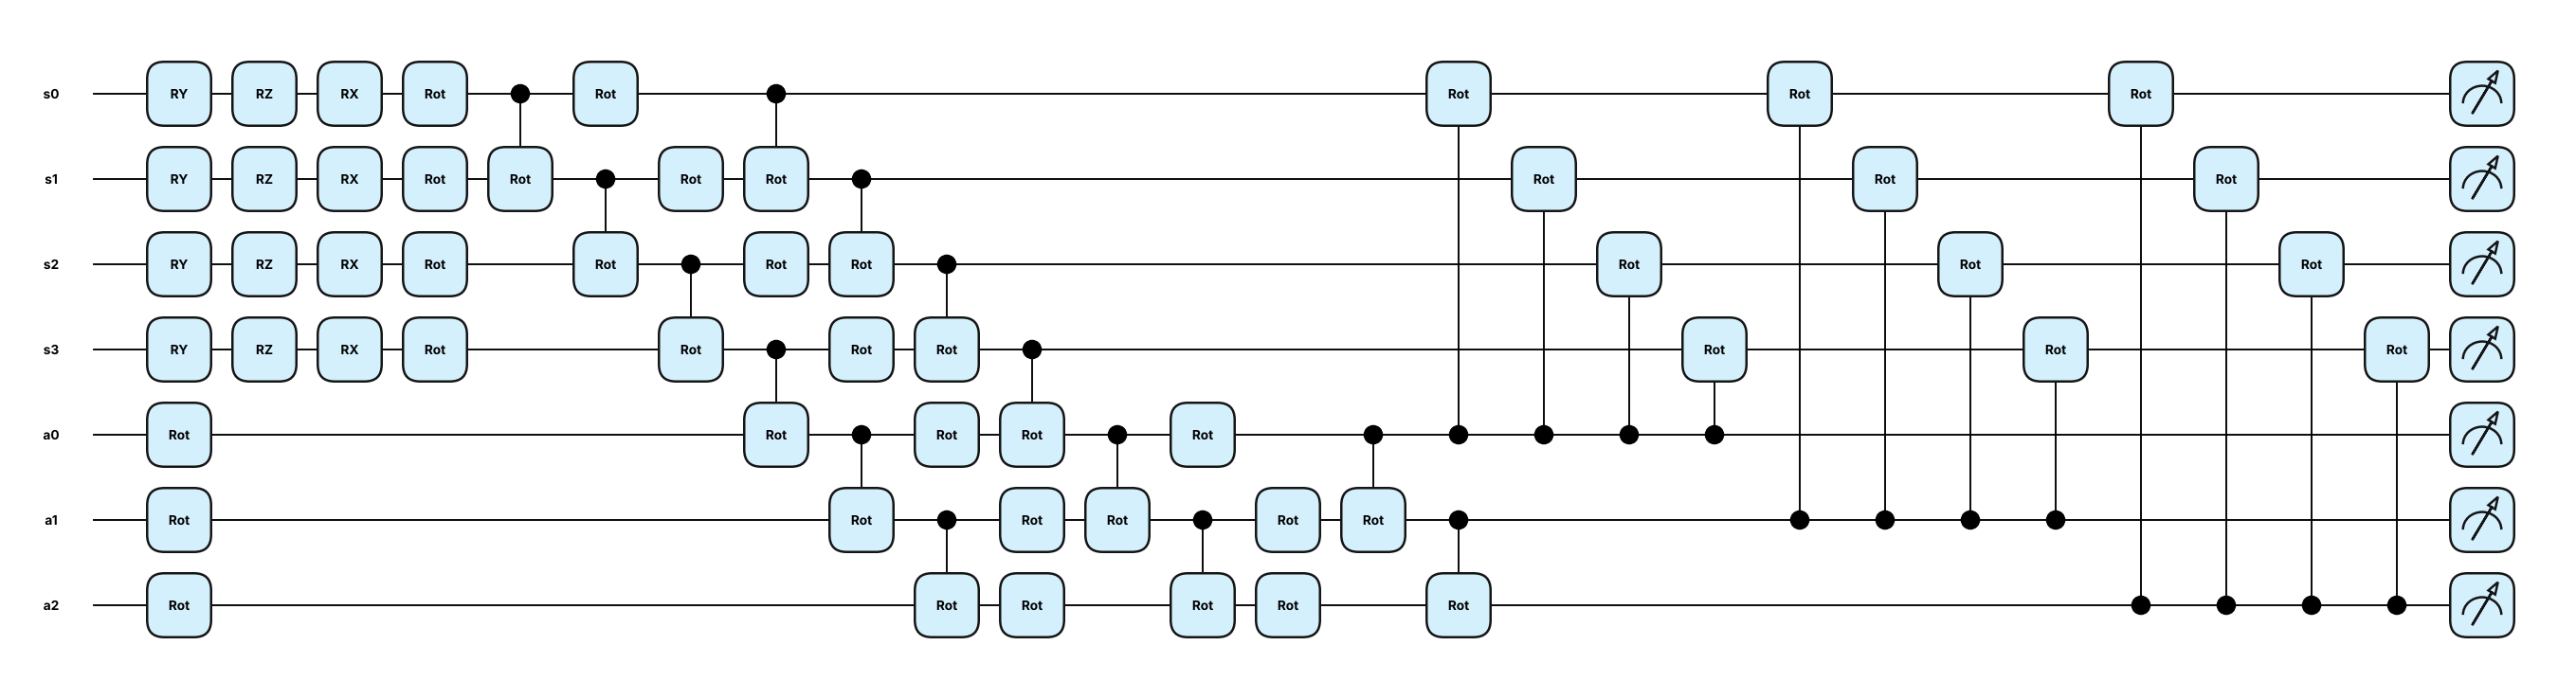
\includegraphics[width=\textwidth]{figures/circuit_one_patch.png}
  \caption{PennyLane drawing of the gates of one patch with $L=2$ repetitions of $W_i$ (the experiments use $L=2$ and $L=4$).}
  \label{fig:onepatch}
\end{figure}

\subsection{MNIST results}

Supplementary Tables~\ref{tab:mnist-results} and~\ref{tab:mnist-amp} give the test accuracies behind Figs.~\ref{fig:capacity} and~\ref{fig:classical}.

\begin{table}[htbp]
  \centering
  \caption{MNIST test accuracy (\%) at the last epoch, mean $\pm$ standard deviation over three seeds. Classical models are sized to the parameter count of the circuit with the given $L$; logistic regression does not depend on $L$. The best mean of each column within each block is in bold. $^\dagger$One of the three seeds stalled at about 47\% training accuracy and is included in the mean. Generated from the result files by \texttt{scripts/paper\_figures.py}.}
  \label{tab:mnist-results}
  \footnotesize
  \setlength{\tabcolsep}{3pt}
  \resizebox{\textwidth}{!}{% generated by scripts/paper_figures.py -- do not edit
\begin{tabular}{@{}lcccccccc@{}}
\toprule
 & \multicolumn{2}{c}{3 vs 5} & \multicolumn{2}{c}{4 vs 9} & \multicolumn{2}{c}{4 classes (0-3)} & \multicolumn{2}{c}{10 classes} \\
\cmidrule(lr){2-3}\cmidrule(lr){4-5}\cmidrule(lr){6-7}\cmidrule(lr){8-9}
 & $8{\times}8$ & $14{\times}14$ & $8{\times}8$ & $14{\times}14$ & $8{\times}8$ & $14{\times}14$ & $8{\times}8$ & $14{\times}14$ \\
\midrule
\multicolumn{9}{@{}l}{\emph{$L=2$ (classical models sized to the circuit with $L=2$)}} \\
serialized, coherent & $96.2\pm0.5$ & $96.9\pm0.2$ & $94.3\pm0.3$ & $96.3\pm0.5$ & $97.4\pm0.2$ & $97.7\pm0.2$ & $89.9\pm0.1$ & $91.8\pm0.2$ \\
serialized, measured & $95.7\pm0.5$ & $96.8\pm0.6$ & $92.6\pm0.4$ & $96.1\pm0.3$ & $90.7\pm4.8$ & $97.0\pm0.1$ & $64.0\pm14.1$$^\dagger$ & $79.9\pm2.8$ \\
MLP, same parameters & $95.6\pm0.1$ & $97.2\pm1.5$ & $95.8\pm0.1$ & $97.3\pm0.6$ & $97.7\pm0.3$ & $98.0\pm0.1$ & $92.0\pm0.2$ & $93.7\pm0.3$ \\
CNN, same parameters & $\mathbf{98.2}\pm0.2$ & $\mathbf{98.5}\pm0.3$ & $\mathbf{96.4}\pm0.2$ & $\mathbf{98.7}\pm0.2$ & $\mathbf{98.7}\pm0.1$ & $\mathbf{99.0}\pm0.1$ & $\mathbf{93.6}\pm0.5$ & $\mathbf{96.3}\pm0.1$ \\
logistic regression & $95.1\pm0.2$ & $95.7\pm0.5$ & $94.8\pm0.2$ & $97.0\pm0.3$ & $97.1\pm0.1$ & $97.5\pm0.1$ & $89.9\pm0.1$ & $91.7\pm0.1$ \\
\midrule
\multicolumn{9}{@{}l}{\emph{$L=4$ (classical models sized to the circuit with $L=4$)}} \\
serialized, coherent & $97.2\pm0.3$ & $97.5\pm0.2$ & $94.9\pm0.3$ & $97.0\pm0.6$ & $97.0\pm0.1$ & $97.8\pm0.3$ & $91.1\pm0.3$ & $92.8\pm0.4$ \\
serialized, measured & $96.9\pm0.2$ & $97.0\pm0.6$ & $94.8\pm0.4$ & $96.8\pm0.3$ & $96.3\pm0.6$ & $97.5\pm0.2$ & $81.2\pm4.1$ & $86.2\pm3.3$ \\
MLP, same parameters & $97.7\pm0.7$ & $98.0\pm0.6$ & $96.8\pm0.3$ & $97.7\pm0.4$ & $98.3\pm0.2$ & $98.3\pm0.0$ & $94.7\pm0.3$ & $95.1\pm0.1$ \\
CNN, same parameters & $\mathbf{98.4}\pm0.4$ & $\mathbf{98.7}\pm0.1$ & $\mathbf{97.0}\pm0.4$ & $\mathbf{98.9}\pm0.2$ & $\mathbf{98.8}\pm0.0$ & $\mathbf{99.1}\pm0.1$ & $\mathbf{95.3}\pm0.2$ & $\mathbf{97.2}\pm0.2$ \\
\bottomrule
\end{tabular}
}
\end{table}

\begin{table}[htbp]
  \centering
  \caption{MNIST test accuracy (\%) of the amplitude-encoding circuits: the whole image as a normalized amplitude vector of 4 qubits (shrunk to $4\times4$) or 7 qubits ($8\times8$ as it is, $14\times14$ shrunk to $11\times11$), followed by $L$ layers of the block of the serialized circuit and the same readout (60--462 parameters). Mean $\pm$ standard deviation over three seeds; the best mean of each column is in bold.}
  \label{tab:mnist-amp}
  \footnotesize
  \setlength{\tabcolsep}{3pt}
  % generated by scripts/paper_figures.py -- do not edit
\begin{tabular}{@{}llcccccccc@{}}
\toprule
 & & \multicolumn{2}{c}{3 vs 5} & \multicolumn{2}{c}{4 vs 9} & \multicolumn{2}{c}{4 classes (0-3)} & \multicolumn{2}{c}{10 classes} \\
\cmidrule(lr){3-4}\cmidrule(lr){5-6}\cmidrule(lr){7-8}\cmidrule(lr){9-10}
qubits & $L$ & $8{\times}8$ & $14{\times}14$ & $8{\times}8$ & $14{\times}14$ & $8{\times}8$ & $14{\times}14$ & $8{\times}8$ & $14{\times}14$ \\
\midrule
4 & 2 & $93.6\pm0.7$ & $93.8\pm0.4$ & $78.0\pm0.6$ & $83.5\pm0.3$ & $88.7\pm0.1$ & $89.2\pm1.1$ & $68.8\pm0.1$ & $72.1\pm1.4$ \\
4 & 4 & $93.9\pm0.2$ & $94.6\pm0.2$ & $79.0\pm1.8$ & $85.0\pm0.4$ & $89.1\pm0.3$ & $90.6\pm0.1$ & $70.5\pm0.7$ & $75.6\pm0.6$ \\
4 & 8 & $94.4\pm0.4$ & $94.6\pm0.2$ & $79.7\pm0.5$ & $85.3\pm1.0$ & $90.0\pm0.4$ & $90.9\pm0.4$ & $72.4\pm0.3$ & $76.4\pm0.9$ \\
\midrule
7 & 2 & $93.5\pm1.4$ & $92.3\pm0.2$ & $88.4\pm0.4$ & $94.9\pm0.4$ & $96.0\pm0.2$ & $96.0\pm0.1$ & $82.4\pm1.2$ & $82.9\pm1.5$ \\
7 & 4 & $94.9\pm1.0$ & $94.6\pm0.8$ & $90.2\pm0.1$ & $\mathbf{95.2}\pm0.1$ & $96.6\pm0.4$ & $96.8\pm0.4$ & $86.3\pm0.2$ & $86.4\pm1.0$ \\
7 & 8 & $\mathbf{96.0}\pm0.5$ & $\mathbf{95.7}\pm0.5$ & $\mathbf{93.5}\pm0.6$ & $\mathbf{95.2}\pm0.5$ & $\mathbf{97.5}\pm0.2$ & $\mathbf{97.1}\pm0.2$ & $\mathbf{87.9}\pm0.4$ & $\mathbf{89.2}\pm0.5$ \\
\bottomrule
\end{tabular}

\end{table}

\subsection{Twelve further datasets}

Supplementary Table~\ref{tab:datasets} describes the datasets and Supplementary Table~\ref{tab:bench} gives the test accuracies behind Fig.~\ref{fig:bench}.

\begin{table}[htbp]
  \centering
  \caption{The twelve further datasets. $d$: features, $N$: patches of four features, $k$: classes. Tabular sets keep their natural class frequencies (majority class in the last column); the image sets are class balanced except PneumoniaMNIST, which keeps its official splits.}
  \label{tab:datasets}
  \footnotesize
  \resizebox{\textwidth}{!}{%
  \begin{tabular}{@{}llrrrrr@{}}
    \toprule
    dataset & source & $d$ & $N$ & $k$ & train / val / test & majority \\
    \midrule
    Waveform & UCI 107~\cite{uci_waveform} (21 wave attributes) & 21 & 6 & 3 & 3\,601 / 400 / 999 & 33.9\% \\
    Wall-Following & UCI 194~\cite{freire2009wall}, 24 sensors & 24 & 6 & 4 & 3\,929 / 436 / 1\,091 & 40.4\% \\
    Covertype & UCI 31~\cite{uci_covertype,blackard1999covertype} & 54 & 14 & 7 & 10\,000 / 2\,000 / 9\,999 & 48.8\% \\
    Letter & UCI 59~\cite{frey1991letter} & 16 & 4 & 26 & 10\,000 / 1\,600 / 4\,000 & 4.1\% \\
    Spambase & UCI 94~\cite{uci_spambase} & 57 & 15 & 2 & 3\,313 / 368 / 920 & 60.5\% \\
    Credit Default & UCI 350~\cite{yeh2009credit} & 23 & 6 & 2 & 10\,000 / 2\,000 / 6\,000 & 77.9\% \\
    Landsat & UCI 146~\cite{uci_landsat,king1995statlog} (train and test joined) & 36 & 9 & 6 & 4\,634 / 514 / 1\,287 & 23.9\% \\
    Dry Bean & UCI 602~\cite{koklu2020drybean} & 16 & 4 & 7 & 9\,801 / 1\,089 / 2\,721 & 26.1\% \\
    \midrule
    Fashion-MNIST & \cite{xiao2017fashion}, $14\times14$ & 196 & 49 & 10 & 10\,000 / 2\,000 / 10\,000 & 10\% \\
    BloodMNIST & MedMNIST v2~\cite{yang2023medmnist,acevedo2020blood}, grayscale, $14\times14$ & 196 & 49 & 8 & 8\,779 / 1\,527 / 3\,421 & 19.5\% \\
    PneumoniaMNIST & MedMNIST v2~\cite{yang2023medmnist,kermany2018pneumonia}, $14\times14$ & 196 & 49 & 2 & 4\,708 / 524 / 624 & 62.5\% \\
    Kuzushiji-MNIST & \cite{clanuwat2018kmnist}, $14\times14$ & 196 & 49 & 10 & 10\,000 / 2\,000 / 10\,000 & 10\% \\
    \bottomrule
  \end{tabular}}
\end{table}

\begin{table}[htbp]
  \centering
  \caption{Test accuracy (\%) on twelve further datasets at the last epoch, mean $\pm$ standard deviation over three seeds; the best mean of each row is in bold. $k$: classes, $N$: patches of four features, params: parameters of the circuit with coherent memory and $L=4$, which is also the size of the MLP and the CNN. Amplitude: the whole input as the amplitude vector of the same seven qubits with $L=4$ or $8$ layers of the same block (200--550 parameters). Gradient boosting: scikit-learn histogram gradient boosting, an ensemble of 300 trees shown as a reference, not tuned. Measured memory was run on the tabular sets only (above the line).}
  \label{tab:bench}
  \footnotesize
  \setlength{\tabcolsep}{2.5pt}
  \resizebox{\textwidth}{!}{% generated by scripts/paper_figures.py -- do not edit
\begin{tabular}{@{}lrrrrrrrrrrr@{}}
\toprule
 & & & & \multicolumn{4}{c}{classical} & \multicolumn{2}{c}{amplitude, 7 qubits} & \multicolumn{2}{c@{}}{serialized, 7 qubits} \\
\cmidrule(lr){5-8}\cmidrule(lr){9-10}\cmidrule(l){11-12}
dataset & $k$ & $N$ & params & logistic & MLP & CNN & grad.\ boost. & $L{=}4$ & $L{=}8$ & \multicolumn{1}{c}{coherent} & \multicolumn{1}{c@{}}{measured} \\
\midrule
Waveform & 3 & 6 & 1056 & $\mathbf{87.2}${\scriptsize$\pm0.1$} & $87.1${\scriptsize$\pm0.8$} & -- & $85.5${\scriptsize$\pm0.5$} & $86.2${\scriptsize$\pm0.2$} & $86.8${\scriptsize$\pm0.6$} & $85.0${\scriptsize$\pm0.2$} & $82.7${\scriptsize$\pm3.1$} \\
Wall-Following & 4 & 6 & 1071 & $68.3${\scriptsize$\pm0.3$} & $91.9${\scriptsize$\pm0.4$} & -- & $\mathbf{99.9}${\scriptsize$\pm0.0$} & $73.0${\scriptsize$\pm1.4$} & $77.1${\scriptsize$\pm1.5$} & $90.1${\scriptsize$\pm0.7$} & $87.0${\scriptsize$\pm2.0$} \\
Covertype & 7 & 14 & 2364 & $71.6${\scriptsize$\pm0.1$} & $75.8${\scriptsize$\pm0.2$} & -- & $\mathbf{82.2}${\scriptsize$\pm0.2$} & $71.7${\scriptsize$\pm0.5$} & $72.0${\scriptsize$\pm0.3$} & $73.8${\scriptsize$\pm0.2$} & $71.7${\scriptsize$\pm0.5$} \\
Letter & 26 & 4 & 1089 & $72.6${\scriptsize$\pm0.2$} & $80.4${\scriptsize$\pm0.8$} & -- & $\mathbf{95.3}${\scriptsize$\pm0.1$} & $59.7${\scriptsize$\pm2.5$} & $63.6${\scriptsize$\pm0.8$} & $71.0${\scriptsize$\pm1.6$} & $63.5${\scriptsize$\pm3.1$} \\
Spambase & 2 & 15 & 2445 & $92.0${\scriptsize$\pm0.1$} & $93.4${\scriptsize$\pm0.5$} & -- & $\mathbf{96.1}${\scriptsize$\pm0.3$} & $90.0${\scriptsize$\pm0.4$} & $90.7${\scriptsize$\pm0.8$} & $91.7${\scriptsize$\pm0.4$} & $93.5${\scriptsize$\pm0.6$} \\
Credit Default & 2 & 6 & 1041 & $81.1${\scriptsize$\pm0.1$} & $81.7${\scriptsize$\pm0.1$} & -- & $81.4${\scriptsize$\pm0.3$} & $79.6${\scriptsize$\pm0.2$} & $79.7${\scriptsize$\pm0.1$} & $81.9${\scriptsize$\pm0.3$} & $\mathbf{82.4}${\scriptsize$\pm0.1$} \\
Landsat & 6 & 9 & 1569 & $82.3${\scriptsize$\pm0.2$} & $89.2${\scriptsize$\pm0.1$} & -- & $\mathbf{92.3}${\scriptsize$\pm0.5$} & $78.7${\scriptsize$\pm0.2$} & $78.9${\scriptsize$\pm0.2$} & $89.3${\scriptsize$\pm1.2$} & $86.8${\scriptsize$\pm1.0$} \\
Dry Bean & 7 & 4 & 804 & $92.1${\scriptsize$\pm0.0$} & $92.3${\scriptsize$\pm0.1$} & -- & $92.8${\scriptsize$\pm0.2$} & $91.8${\scriptsize$\pm0.1$} & $91.8${\scriptsize$\pm0.2$} & $\mathbf{92.9}${\scriptsize$\pm0.2$} & $92.8${\scriptsize$\pm0.0$} \\
\midrule
Fashion-MNIST & 10 & 49 & 7869 & $82.6${\scriptsize$\pm0.2$} & $85.2${\scriptsize$\pm0.1$} & $85.7${\scriptsize$\pm0.6$} & $\mathbf{86.5}${\scriptsize$\pm0.4$} & $73.7${\scriptsize$\pm0.4$} & $74.4${\scriptsize$\pm0.8$} & $82.7${\scriptsize$\pm0.2$} & -- \\
BloodMNIST & 8 & 49 & 7839 & $67.2${\scriptsize$\pm0.4$} & $70.3${\scriptsize$\pm1.2$} & $81.2${\scriptsize$\pm0.4$} & $\mathbf{86.0}${\scriptsize$\pm0.2$} & $58.0${\scriptsize$\pm0.6$} & $60.2${\scriptsize$\pm0.2$} & $73.8${\scriptsize$\pm1.3$} & -- \\
PneumoniaMNIST & 2 & 49 & 7749 & $83.5${\scriptsize$\pm0.1$} & $84.1${\scriptsize$\pm0.9$} & $85.6${\scriptsize$\pm0.8$} & $84.9${\scriptsize$\pm0.0$} & $81.2${\scriptsize$\pm1.5$} & $81.9${\scriptsize$\pm1.2$} & $\mathbf{87.7}${\scriptsize$\pm0.7$} & -- \\
Kuzushiji-MNIST & 10 & 49 & 7869 & $68.2${\scriptsize$\pm0.3$} & $78.7${\scriptsize$\pm0.2$} & $80.3${\scriptsize$\pm1.5$} & $\mathbf{83.4}${\scriptsize$\pm0.3$} & $58.3${\scriptsize$\pm0.8$} & $62.6${\scriptsize$\pm0.8$} & $70.4${\scriptsize$\pm0.7$} & -- \\
\bottomrule
\end{tabular}
}
\end{table}

\begin{table}[htbp]
  \centering
  \caption{As Supplementary Table~\ref{tab:bench}, but balanced accuracy (\%), the mean of the per-class recalls: last epoch, mean $\pm$ standard deviation over three seeds; the best mean of each row is in bold.}
  \label{tab:bench-bal}
  \footnotesize
  \setlength{\tabcolsep}{2.5pt}
  \resizebox{\textwidth}{!}{% generated by scripts/paper_figures.py -- do not edit
\begin{tabular}{@{}lrrrrrrrrrrr@{}}
\toprule
 & & & & \multicolumn{4}{c}{classical} & \multicolumn{2}{c}{amplitude, 7 qubits} & \multicolumn{2}{c@{}}{serialized, 7 qubits} \\
\cmidrule(lr){5-8}\cmidrule(lr){9-10}\cmidrule(l){11-12}
dataset & $k$ & $N$ & params & logistic & MLP & CNN & grad.\ boost. & $L{=}4$ & $L{=}8$ & \multicolumn{1}{c}{coherent} & \multicolumn{1}{c@{}}{measured} \\
\midrule
Waveform & 3 & 6 & 1056 & $\mathbf{87.2}${\scriptsize$\pm0.1$} & $87.1${\scriptsize$\pm0.8$} & -- & $85.5${\scriptsize$\pm0.5$} & $86.2${\scriptsize$\pm0.2$} & $86.8${\scriptsize$\pm0.6$} & $85.0${\scriptsize$\pm0.2$} & $82.7${\scriptsize$\pm3.1$} \\
Wall-Following & 4 & 6 & 1071 & $59.7${\scriptsize$\pm1.0$} & $90.8${\scriptsize$\pm0.9$} & -- & $\mathbf{99.9}${\scriptsize$\pm0.0$} & $66.2${\scriptsize$\pm1.8$} & $69.9${\scriptsize$\pm0.9$} & $88.8${\scriptsize$\pm0.8$} & $84.6${\scriptsize$\pm2.7$} \\
Covertype & 7 & 14 & 2364 & $46.0${\scriptsize$\pm1.2$} & $56.2${\scriptsize$\pm2.4$} & -- & $\mathbf{67.8}${\scriptsize$\pm0.2$} & $42.3${\scriptsize$\pm0.1$} & $42.1${\scriptsize$\pm1.7$} & $45.3${\scriptsize$\pm1.2$} & $38.1${\scriptsize$\pm2.6$} \\
Letter & 26 & 4 & 1089 & $72.5${\scriptsize$\pm0.2$} & $80.4${\scriptsize$\pm0.8$} & -- & $\mathbf{95.3}${\scriptsize$\pm0.1$} & $59.6${\scriptsize$\pm2.4$} & $63.5${\scriptsize$\pm0.7$} & $70.8${\scriptsize$\pm1.6$} & $63.5${\scriptsize$\pm3.1$} \\
Spambase & 2 & 15 & 2445 & $91.2${\scriptsize$\pm0.1$} & $92.9${\scriptsize$\pm0.4$} & -- & $\mathbf{96.1}${\scriptsize$\pm0.3$} & $89.2${\scriptsize$\pm0.5$} & $90.0${\scriptsize$\pm0.8$} & $91.4${\scriptsize$\pm0.8$} & $93.1${\scriptsize$\pm0.7$} \\
Credit Default & 2 & 6 & 1041 & $61.2${\scriptsize$\pm0.2$} & $65.4${\scriptsize$\pm0.3$} & -- & $65.0${\scriptsize$\pm0.2$} & $58.5${\scriptsize$\pm0.4$} & $59.1${\scriptsize$\pm0.3$} & $65.3${\scriptsize$\pm0.7$} & $\mathbf{66.3}${\scriptsize$\pm0.4$} \\
Landsat & 6 & 9 & 1569 & $74.7${\scriptsize$\pm0.4$} & $86.5${\scriptsize$\pm0.1$} & -- & $\mathbf{90.1}${\scriptsize$\pm0.6$} & $69.3${\scriptsize$\pm0.2$} & $69.4${\scriptsize$\pm0.2$} & $86.8${\scriptsize$\pm1.4$} & $83.6${\scriptsize$\pm1.3$} \\
Dry Bean & 7 & 4 & 804 & $93.4${\scriptsize$\pm0.0$} & $93.5${\scriptsize$\pm0.0$} & -- & $93.8${\scriptsize$\pm0.2$} & $92.9${\scriptsize$\pm0.2$} & $93.0${\scriptsize$\pm0.1$} & $\mathbf{93.9}${\scriptsize$\pm0.2$} & $93.8${\scriptsize$\pm0.1$} \\
\midrule
Fashion-MNIST & 10 & 49 & 7869 & $82.6${\scriptsize$\pm0.2$} & $85.2${\scriptsize$\pm0.1$} & $85.7${\scriptsize$\pm0.6$} & $\mathbf{86.5}${\scriptsize$\pm0.4$} & $73.7${\scriptsize$\pm0.4$} & $74.4${\scriptsize$\pm0.8$} & $82.7${\scriptsize$\pm0.2$} & -- \\
BloodMNIST & 8 & 49 & 7839 & $67.2${\scriptsize$\pm0.4$} & $69.8${\scriptsize$\pm1.1$} & $79.5${\scriptsize$\pm0.4$} & $\mathbf{84.8}${\scriptsize$\pm0.3$} & $55.5${\scriptsize$\pm0.5$} & $57.4${\scriptsize$\pm1.1$} & $73.0${\scriptsize$\pm1.1$} & -- \\
PneumoniaMNIST & 2 & 49 & 7749 & $78.9${\scriptsize$\pm0.2$} & $79.3${\scriptsize$\pm1.4$} & $81.2${\scriptsize$\pm1.2$} & $80.8${\scriptsize$\pm0.0$} & $76.1${\scriptsize$\pm2.1$} & $77.0${\scriptsize$\pm1.8$} & $\mathbf{84.0}${\scriptsize$\pm1.0$} & -- \\
Kuzushiji-MNIST & 10 & 49 & 7869 & $68.2${\scriptsize$\pm0.3$} & $78.7${\scriptsize$\pm0.2$} & $80.3${\scriptsize$\pm1.5$} & $\mathbf{83.4}${\scriptsize$\pm0.3$} & $58.3${\scriptsize$\pm0.8$} & $62.6${\scriptsize$\pm0.8$} & $70.4${\scriptsize$\pm0.7$} & -- \\
\bottomrule
\end{tabular}
}
\end{table}

\subsection{Classical models with the structure of the circuit}

\begin{table}[htbp]
  \centering
  \caption{The serialized circuit ($L=4$) against classical models that read the input patch by patch with position-specific parameters. Test accuracy (\%) at the last epoch, mean over three seeds; the best mean of each row is in bold. MLP: the one-hidden-layer MLP of Supplementary Table~\ref{tab:bench} (for MNIST, the parameter-matched MLP of Supplementary Table~\ref{tab:mnist-results}). Seq.\ RNN: recurrent network with its own weights at every patch; MPS: matrix-product-state classifier with one tensor per feature; both are sized to the parameter count of the circuit as closely as their hidden or bond dimension allows. 8-state HMM: input-driven hidden Markov model over eight states, with 1.5 to 2 times the parameters of the circuit. The learning rate of each classical model is chosen by mean validation accuracy. Measured memory was not run on the 49-patch image sets.}
  \label{tab:struct}
  \footnotesize
  % generated by scripts/paper_figures.py -- do not edit
\begin{tabular}{@{}lrrrrrr@{}}
\toprule
 & \multicolumn{2}{c}{serialized circuit} & \multicolumn{4}{c@{}}{classical} \\
\cmidrule(lr){2-3}\cmidrule(l){4-7}
dataset & coherent & measured & MLP & seq.\ RNN & MPS & 8-state HMM \\
\midrule
Waveform & $85.0$ & $82.7$ & $87.1$ & $87.4$ & $\mathbf{87.5}$ & $84.9$ \\
Wall-Following & $90.1$ & $87.0$ & $91.9$ & $93.1$ & $\mathbf{95.2}$ & $85.7$ \\
Covertype & $73.8$ & $71.7$ & $\mathbf{75.8}$ & $75.3$ & $75.2$ & $71.3$ \\
Letter & $71.0$ & $63.5$ & $80.4$ & $\mathbf{80.7}$ & $71.4$ & $53.8$ \\
Spambase & $91.7$ & $93.5$ & $93.4$ & $93.2$ & $\mathbf{93.8}$ & $92.5$ \\
Credit Default & $81.9$ & $\mathbf{82.4}$ & $81.7$ & $82.2$ & $82.0$ & $81.9$ \\
Landsat & $89.3$ & $86.8$ & $89.2$ & $\mathbf{89.7}$ & $89.6$ & $83.7$ \\
Dry Bean & $\mathbf{92.9}$ & $92.8$ & $92.3$ & $92.8$ & $\mathbf{92.9}$ & $91.9$ \\
Fashion-MNIST & $82.7$ & -- & $\mathbf{85.2}$ & $77.1$ & $82.2$ & $53.0$ \\
BloodMNIST & $\mathbf{73.8}$ & -- & $70.3$ & $64.7$ & $71.9$ & $44.9$ \\
PneumoniaMNIST & $\mathbf{87.7}$ & -- & $84.1$ & $87.6$ & $87.5$ & $82.9$ \\
Kuzushiji-MNIST & $70.4$ & -- & $\mathbf{78.7}$ & $61.8$ & $62.1$ & $31.0$ \\
MNIST $8\times8$, 3 vs.\ 5 & $97.2$ & $96.9$ & $97.7$ & $\mathbf{98.1}$ & $97.4$ & $65.0$ \\
MNIST $8\times8$, 10 classes & $91.1$ & $81.2$ & $\mathbf{94.7}$ & $92.7$ & $92.1$ & $68.2$ \\
\bottomrule
\end{tabular}

\end{table}

\subsection{Readout and head variants on Letter}

Supplementary Table~\ref{tab:letter} collects the variants of the circuit run on Letter, each against a one-hidden-layer MLP with the same number of parameters.

\begin{table}[htbp]
  \centering
  \caption{Letter (26 classes): readout, head and depth variants of the circuit with coherent memory, against a one-hidden-layer MLP of the same size. Test accuracy (\%), mean $\pm$ standard deviation over three seeds; the better mean of each row is in bold. Gradient-boosted trees reach $95.3\pm0.1$.}
  \label{tab:letter}
  \footnotesize
  % generated by scripts/paper_figures.py -- do not edit
\begin{tabular}{@{}lrlrl@{}}
\toprule
 & \multicolumn{2}{c}{circuit} & \multicolumn{2}{c@{}}{MLP, same size} \\
\cmidrule(lr){2-3}\cmidrule(l){4-5}
readout and head & params & accuracy & params & accuracy \\
\midrule
$Z$, $ZZ$ (14 features), linear head, $L=4$ & 1\,089 & $71.0\pm1.6$ & 1\,101 & $\mathbf{80.4}\pm0.8$ \\
$Z$, $ZZ$ (14 features), linear head, $L=9$ & 1\,869 & $71.8\pm2.1$ & -- & -- \\
$+X$, $XX$, $Y$, $YY$ (42 features), linear head, $L=4$ & 1\,817 & $79.9\pm0.2$ & 1\,832 & $\mathbf{84.7}\pm1.2$ \\
$Z$, $ZZ$ (14 features), MLP head (64 units), $L=4$ & 3\,349 & $85.6\pm0.6$ & 3\,337 & $\mathbf{87.8}\pm0.2$ \\
\bottomrule
\end{tabular}

\end{table}

\subsection{$28\times28$ images}
\label{sec:supp-28}

At $28\times28$ the serialized circuit has 196 patches and 74\% of them are empty (62\% at $14\times14$, 41\% at $8\times8$). With the settings of the MNIST experiments it stays at chance or only fits the training set, and the simulation takes about 47 minutes (3 vs.\ 5) to 2 hours (10 classes) per epoch, i.e.\ days per run, so it is not reported. The classical and amplitude-encoding baselines were run at $28\times28$ and are in the code repository.
